%%%%%%%%%%%%%%%%%%%%%%%%%%%%%%%%%%%%%%%%%
% Final Year Project Report -- Bachelor of Engineering
% University of Glasgow
%
% Student : Siwei Chen
% GUID    : 2839900C
% Year    : 2025--2026
%%%%%%%%%%%%%%%%%%%%%%%%%%%%%%%%%%%%%%%%%

%----------------------------------------------------------------------------------------
%  PACKAGES AND OTHER DOCUMENT CONFIGURATIONS
%----------------------------------------------------------------------------------------

\documentclass[
12pt,
oneside,
singlespacing,
parskip,
]{article}

\usepackage{geometry}
\usepackage{natbib}
\usepackage[utf8]{inputenc}
\usepackage[T1]{fontenc}
\usepackage{mathptmx}
\usepackage{color}
\usepackage[scaled]{helvet}
\usepackage{courier}
\usepackage{textcomp}
\usepackage{graphicx}
\usepackage{hyperref}

% Additional packages for technical content
\usepackage{amsmath,amssymb,amsthm}
\usepackage{booktabs}
\usepackage{multirow}
\usepackage{float}
\usepackage{caption}
\usepackage{subcaption}
\usepackage{xcolor}
\usepackage{enumitem}
\usepackage{algorithm}
\usepackage{algpseudocode}
\usepackage{listings}
\usepackage{array}
\usepackage{tabularx}

\graphicspath{{figures/}{./figures/}{./}}

%----------------------------------------------------------------------------------------
%  THEOREM ENVIRONMENTS
%----------------------------------------------------------------------------------------
\newtheorem{theorem}{Theorem}[section]
\newtheorem{definition}{Definition}[section]
\newtheorem{lemma}{Lemma}[section]
\newtheorem{corollary}{Corollary}[section]

%----------------------------------------------------------------------------------------
%  CODE LISTING STYLE
%----------------------------------------------------------------------------------------
\lstset{
  language=Python,
  basicstyle=\ttfamily\small,
  keywordstyle=\color{blue}\bfseries,
  commentstyle=\color{gray}\itshape,
  stringstyle=\color{red!70!black},
  numbers=left,
  numberstyle=\tiny\color{gray},
  numbersep=5pt,
  frame=single,
  breaklines=true,
  breakatwhitespace=true,
  tabsize=4,
  showstringspaces=false,
  captionpos=b,
  aboveskip=10pt,
  belowskip=10pt,
}

%----------------------------------------------------------------------------------------
%  THESIS INFORMATION
%----------------------------------------------------------------------------------------

\newcommand{\thesistitle}{Design and Analysis of a Double-Layer HotStuff Consensus Protocol: Reliability Modelling and Experimental Evaluation}
\newcommand{\GUID}{2839900C}
\newcommand{\student}{Siwei \textsc{Chen}}
\newcommand{\firstsupervisor}{[Supervisor Name]}
\newcommand{\secondsupervisor}{[Co-Supervisor Name]}
\newcommand{\degree}{Engineering}
\newcommand{\subject}{Computing Science}
\newcommand{\keywords}{Byzantine Fault Tolerance, HotStuff, Consensus Protocol, Reliability, Monte Carlo Simulation}
\newcommand{\university}{\href{https://www.gla.ac.uk/}{University of Glasgow}}
\newcommand{\department}{\href{https://www.gla.ac.uk/schools/computing/}{School of Computing Science}}

%----------------------------------------------------------------------------------------
%  CUSTOM ENVIRONMENTS
%----------------------------------------------------------------------------------------

\newenvironment{declaration}{
    \newgeometry{left=4em,right=4em,bottom=6em,top=6em}
    \addcontentsline{toc}{section}{Coursework Declaration and Feedback Form}
    }{\clearpage\restoregeometry}

\renewenvironment{abstract}{
    \section*{Abstract}
    \bigskip
    \addcontentsline{toc}{section}{Abstract}}{\clearpage}

\newenvironment{acknowledgement}{
    \section*{Acknowledgements}
    \bigskip
    \addcontentsline{toc}{section}{Acknowledgements}}{\clearpage}

\geometry{
    paper=a4paper,
    inner=6em,
    outer=6em,
    bindingoffset=0em,
    top=6em,
    bottom=6em,
}

\hypersetup{colorlinks=true,linkcolor=black,citecolor=black,urlcolor=black}
\AtBeginDocument{
\hypersetup{pdftitle=\thesistitle}
\hypersetup{pdfauthor=\student}
\hypersetup{pdfkeywords=\keywords}
}

%========================================================================================
\begin{document}
%========================================================================================

\pagestyle{plain}

%----------------------------------------------------------------------------------------
%  TITLE PAGE
%----------------------------------------------------------------------------------------

\begin{titlepage}
\begin{flushleft}
  \noindent\includegraphics[width=0.25\linewidth]{logo_jw_eng}\\[5ex]
\end{flushleft}

\begin{center}

\textsc{\Large Final Year Project Report\\Bachelor of Engineering}\\[2cm]

{\huge \bfseries \thesistitle\par}\vspace{3cm}

\begin{minipage}[t]{0.4\textwidth}
\begin{center} \huge
\student\\
\vspace*{.02\textheight}
\GUID\\
\end{center}
\end{minipage}\\[3cm]

\vfill

{\huge 2025--2026}\\[2cm]

\end{center}
\end{titlepage}

\pagenumbering{roman}

%----------------------------------------------------------------------------------------
%  DECLARATION PAGE
%----------------------------------------------------------------------------------------
\renewcommand{\arraystretch}{1.3}
\begin{declaration}
\begin{table}[h!]
    \resizebox{\textwidth}{!}{
    \begin{tabular}{|p{6.5cm}|l|}
    \hline
    Student Name: \student & Student GUID: \GUID \\ \hline
    \begin{tabular}[c]{@{}l@{}}Course Code :\\ ENG4110P\end{tabular} & \begin{tabular}[c]{@{}l@{}}Course Name :\\ INDIVIDUAL PROJECT 4\end{tabular} \\ \hline
    \begin{tabular}[c]{@{}l@{}}Name of 1st Supervisor:\\ \firstsupervisor \end{tabular} & \begin{tabular}[c]{@{}l@{}}Name of 2nd Supervisor:\\ \secondsupervisor \end{tabular} \\ \hline
    \multicolumn{2}{|l|}{\begin{tabular}[c]{@{}l@{}}Title of Project:\\{\large\textbf{\thesistitle}} \end{tabular}} \\ \hline
    \end{tabular}
    }
\end{table}

\bigskip

\section*{Declaration of Originality and Submission Information}
\begin{quote}
  I affirm that this submission is all my own work in accordance with the University of Glasgow Regulations and the School of Computing Science requirements.
\end{quote}

\end{declaration}

%----------------------------------------------------------------------------------------
%  ABSTRACT
%----------------------------------------------------------------------------------------

\begin{abstract}
Byzantine Fault-Tolerant (BFT) consensus protocols are foundational to distributed systems, blockchains, and safety-critical applications. However, achieving high reliability under realistic network conditions---where messages are lost with non-negligible probability---remains a key challenge, particularly as system size scales.

This project designs, implements, and evaluates a \emph{double-layer HotStuff} consensus protocol, in which $N$ nodes are organised into $K = \mathrm{round}(\sqrt{N})$ groups arranged in a two-tier hierarchy. An interactive web-based demonstration platform (built with Vue~3 and FastAPI) allows real-time observation of the consensus process, including Byzantine behaviour scenarios. A Monte Carlo simulation engine then systematically evaluates the system across 301 experimental configurations covering node counts $N = 16$--$100$ and message delivery rates $p = 90\%$--$99\%$, each run for 1000 rounds.

The experiments reveal a surprising \emph{non-monotonic oscillation} in reliability as a function of $N$: adding more nodes can \emph{decrease} reliability, violating naive scalability intuition. We derive a closed-form probabilistic model explaining this oscillation through the interaction of three discrete staircase functions---the group count $K$, the group size $g$, and the local quorum threshold $q_\mathrm{local}$---termed the ``Three Gears'' mechanism. A single calibrated exponent $\alpha \approx 3.73$ captures multi-hop delivery effects, and the model achieves Pearson correlation $R = 0.80$ against experimental data. A practical design guideline emerges: choosing $N$ at or near perfect-square values (e.g., $N \in \{25, 36, 49, 64, 81, 100\}$) maximises reliability for a given delivery rate.
\end{abstract}

%----------------------------------------------------------------------------------------
%  ACKNOWLEDGEMENTS
%----------------------------------------------------------------------------------------

\begin{acknowledgement}
I would like to express my sincere gratitude to my supervisors for their guidance and support throughout this project. I am also grateful to the School of Computing Science for providing the computational resources necessary to conduct the large-scale Monte Carlo experiments. Finally, I would like to thank my fellow students for helpful discussions on distributed systems theory.
\end{acknowledgement}

%----------------------------------------------------------------------------------------
%  TABLE OF CONTENTS
%----------------------------------------------------------------------------------------
\tableofcontents
\pagebreak

%----------------------------------------------------------------------------------------
%  MAIN CONTENT
%----------------------------------------------------------------------------------------

\pagestyle{plain}
\pagenumbering{arabic}

%========================================================================================
\section{Introduction}
\label{sec:intro}
%========================================================================================

\subsection{Motivation}

Distributed consensus is the problem of getting a set of independent processes---nodes in a network---to agree on a single value, even when some nodes may behave maliciously. This problem underlies modern blockchains \citep{nakamoto2008bitcoin}, distributed databases \citep{lamport2001paxos}, and safety-critical control systems. The Byzantine Generals Problem, formalised by \citet{lamport1982byzantine}, established that consensus is achievable so long as the number of faulty nodes $f$ satisfies $f < N/3$, where $N$ is the total number of nodes.

Early BFT protocols such as PBFT \citep{castro1999practical} achieve theoretical safety and liveness but suffer from $O(N^2)$ message complexity, making them impractical for large networks. HotStuff \citep{yin2019hotstuff}, introduced by Yin et al., reduces this to $O(N)$ per phase by routing all votes through a designated leader, while maintaining the same BFT safety guarantees. However, in real networks, messages can be dropped, delayed, or corrupted. The impact of such \emph{message delivery imperfection} on the reliability of HotStuff-based protocols at scale is not well characterised.

A natural approach to improving scalability and fault localisation is to organise nodes into a \emph{two-tier hierarchy}: groups of nodes first reach local consensus, and group representatives then participate in global consensus. This \emph{double-layer} (or multi-layer) architecture reduces the number of participants in each voting step, potentially improving throughput and resilience \citep{buterin2017casper}. However, it introduces new parameters---group count $K$, group size $g$, and local quorum threshold $q_\mathrm{local}$---whose interactions under unreliable networks are not understood.

\subsection{Aims and Objectives}

This project addresses the following research questions:

\begin{enumerate}
  \item How does reliability of a double-layer HotStuff protocol vary with node count $N$ and message delivery rate $p$ under a realistic network loss model?
  \item Can a closed-form mathematical model predict this reliability, and what are the key parameters driving it?
  \item What design guidelines can be derived for choosing $N$ and $K$ to maximise reliability?
\end{enumerate}

To answer these questions, the project delivers:

\begin{itemize}
  \item An \textbf{interactive web platform} for real-time demonstration and experimentation with double-layer HotStuff, supporting configurable Byzantine fault scenarios.
  \item A \textbf{Monte Carlo simulation engine} capable of evaluating reliability across hundreds of parameter configurations.
  \item A \textbf{probabilistic reliability model} derived from first principles and validated against simulation data.
\end{itemize}

\subsection{Report Structure}

Section~\ref{sec:background} reviews BFT consensus and HotStuff. Section~\ref{sec:design} describes the system architecture and implementation. Section~\ref{sec:methodology} defines the experimental methodology. Section~\ref{sec:results} presents the experimental results. Section~\ref{sec:model} derives the mathematical model. Section~\ref{sec:discussion} discusses the scaling paradox and design recommendations. Section~\ref{sec:conclusions} concludes.

%========================================================================================
\section{Background and Related Work}
\label{sec:background}
%========================================================================================

\subsection{Byzantine Fault Tolerance}

A distributed system is \emph{Byzantine fault-tolerant} if it continues to operate correctly even when up to $f$ nodes behave arbitrarily---including lying, sending conflicting messages, or remaining silent \citep{lamport1982byzantine}. The fundamental lower bound states that BFT consensus requires $N \geq 3f + 1$ nodes \citep{fischer1985impossibility}.

\subsection{PBFT}

Practical Byzantine Fault Tolerance (PBFT) \citep{castro1999practical} was the first efficient BFT protocol suitable for practical deployment. It operates in a three-phase pipeline: \emph{pre-prepare}, \emph{prepare}, and \emph{commit}. Each phase requires $2f + 1$ matching messages from distinct nodes before proceeding. Its main limitation is $O(N^2)$ message complexity per consensus round, which limits scalability to tens of nodes.

\subsection{HotStuff}

HotStuff \citep{yin2019hotstuff} achieves $O(N)$ message complexity per phase by introducing a \emph{leader-centric} design: all nodes send their votes to the current leader, who aggregates them into a \emph{Quorum Certificate} (QC) and broadcasts the QC. This reduces each phase to one broadcast and $N$ unicasts. HotStuff uses a four-phase pipeline:

\begin{enumerate}
  \item \textbf{Prepare}: Leader proposes a value; all nodes vote to the leader.
  \item \textbf{Pre-Commit}: Leader broadcasts Prepare-QC; nodes vote again.
  \item \textbf{Commit}: Leader broadcasts Pre-Commit-QC; nodes commit.
  \item \textbf{Decide}: Leader broadcasts Commit-QC; consensus is decided.
\end{enumerate}

Safety is guaranteed by the \emph{SafeNode} predicate: a node only votes for a proposal if $\mathrm{proposal.view} > \mathrm{lockedQC.view}$ or the proposal extends the locked QC. Liveness is provided by a \emph{View Change} mechanism that rotates the leader when a timeout occurs.

\subsection{Multi-Layer Consensus}

Several recent works have explored hierarchical consensus to improve scalability. Ethereum's Casper \citep{buterin2017casper} uses a two-layer finality mechanism. Tendermint \citep{buchman2016tendermint} and its derivatives organise validators into committees. The work most closely related to ours is the hierarchical BFT approach of \citet{david2018ouroboros}, which partitions nodes into groups and uses a two-round aggregation process. However, none of these works provide a closed-form analysis of how reliability varies with group structure under message loss.

\subsection{Reliability Under Message Loss}

The effect of message loss on BFT protocols has been studied in the context of network partitions \citep{brewer2000cap} and asynchronous networks \citep{fischer1985impossibility}. However, the specific impact of \emph{uniform Bernoulli message loss} on the reliability of hierarchical HotStuff has not been previously modelled analytically. Our work fills this gap.

%========================================================================================
\section{System Design and Implementation}
\label{sec:design}
%========================================================================================

\subsection{Overall Architecture}

The system consists of two major components:

\begin{enumerate}
  \item A \textbf{web-based interactive platform} for real-time consensus demonstration with human and robot participants.
  \item A \textbf{headless Monte Carlo simulation engine} for automated large-scale reliability experiments.
\end{enumerate}

Both components share the same backend consensus logic, ensuring experimental fidelity.

The technology stack is:
\begin{itemize}
  \item \textbf{Frontend}: Vue~3, Element Plus, Pinia, Vue Router, Socket.IO Client, ECharts.
  \item \textbf{Backend}: FastAPI, python-socketio, Pydantic, Uvicorn.
  \item \textbf{Persistence}: SQLite (session state and consensus history).
\end{itemize}

\subsection{Double-Layer HotStuff Protocol}

\subsubsection{Topology}

The $N$ nodes are partitioned into $K = \mathrm{round}(\sqrt{N})$ groups using a fair partition (Algorithm~\ref{alg:partition}). The first $(N \bmod K)$ groups receive $\lceil N/K \rceil$ nodes; the remainder receive $\lfloor N/K \rfloor$ nodes.

\begin{algorithm}[H]
\caption{Fair group partition}
\label{alg:partition}
\begin{algorithmic}[1]
\Require Node count $N$, group count $K$
\Ensure Assignment $\mathrm{group}[i]$ for each node $i$
\State $\mathrm{base} \leftarrow \lfloor N/K \rfloor$; $\mathrm{rem} \leftarrow N \bmod K$
\State $\mathrm{start} \leftarrow 0$
\For{$g = 0$ to $K-1$}
    \State $\mathrm{size} \leftarrow \mathrm{base} + (1 \text{ if } g < \mathrm{rem} \text{ else } 0)$
    \For{$i = \mathrm{start}$ to $\mathrm{start}+\mathrm{size}-1$}
        \State $\mathrm{group}[i] \leftarrow g$; $\mathrm{leader}[i] \leftarrow \mathrm{start}$
    \EndFor
    \State $\mathrm{start} \leftarrow \mathrm{start} + \mathrm{size}$
\EndFor
\end{algorithmic}
\end{algorithm}

Each node is assigned one of three roles:
\begin{itemize}
  \item \textbf{Root} (Global Leader): The node with $\mathrm{id} = \mathrm{view} \bmod N$. Coordinates global consensus.
  \item \textbf{Group Leader}: The first node of each non-root group. Aggregates local votes.
  \item \textbf{Member}: All other nodes. Votes within their group.
\end{itemize}

\subsubsection{Consensus Flow}

Figure~\ref{fig:hotstuff_flow} illustrates the seven-step consensus flow in double-layer mode. In single-layer mode (when $K = 1$ or $N$ is small), all nodes communicate directly with the Global Leader, reducing to standard HotStuff.

\begin{figure}[H]
\centering
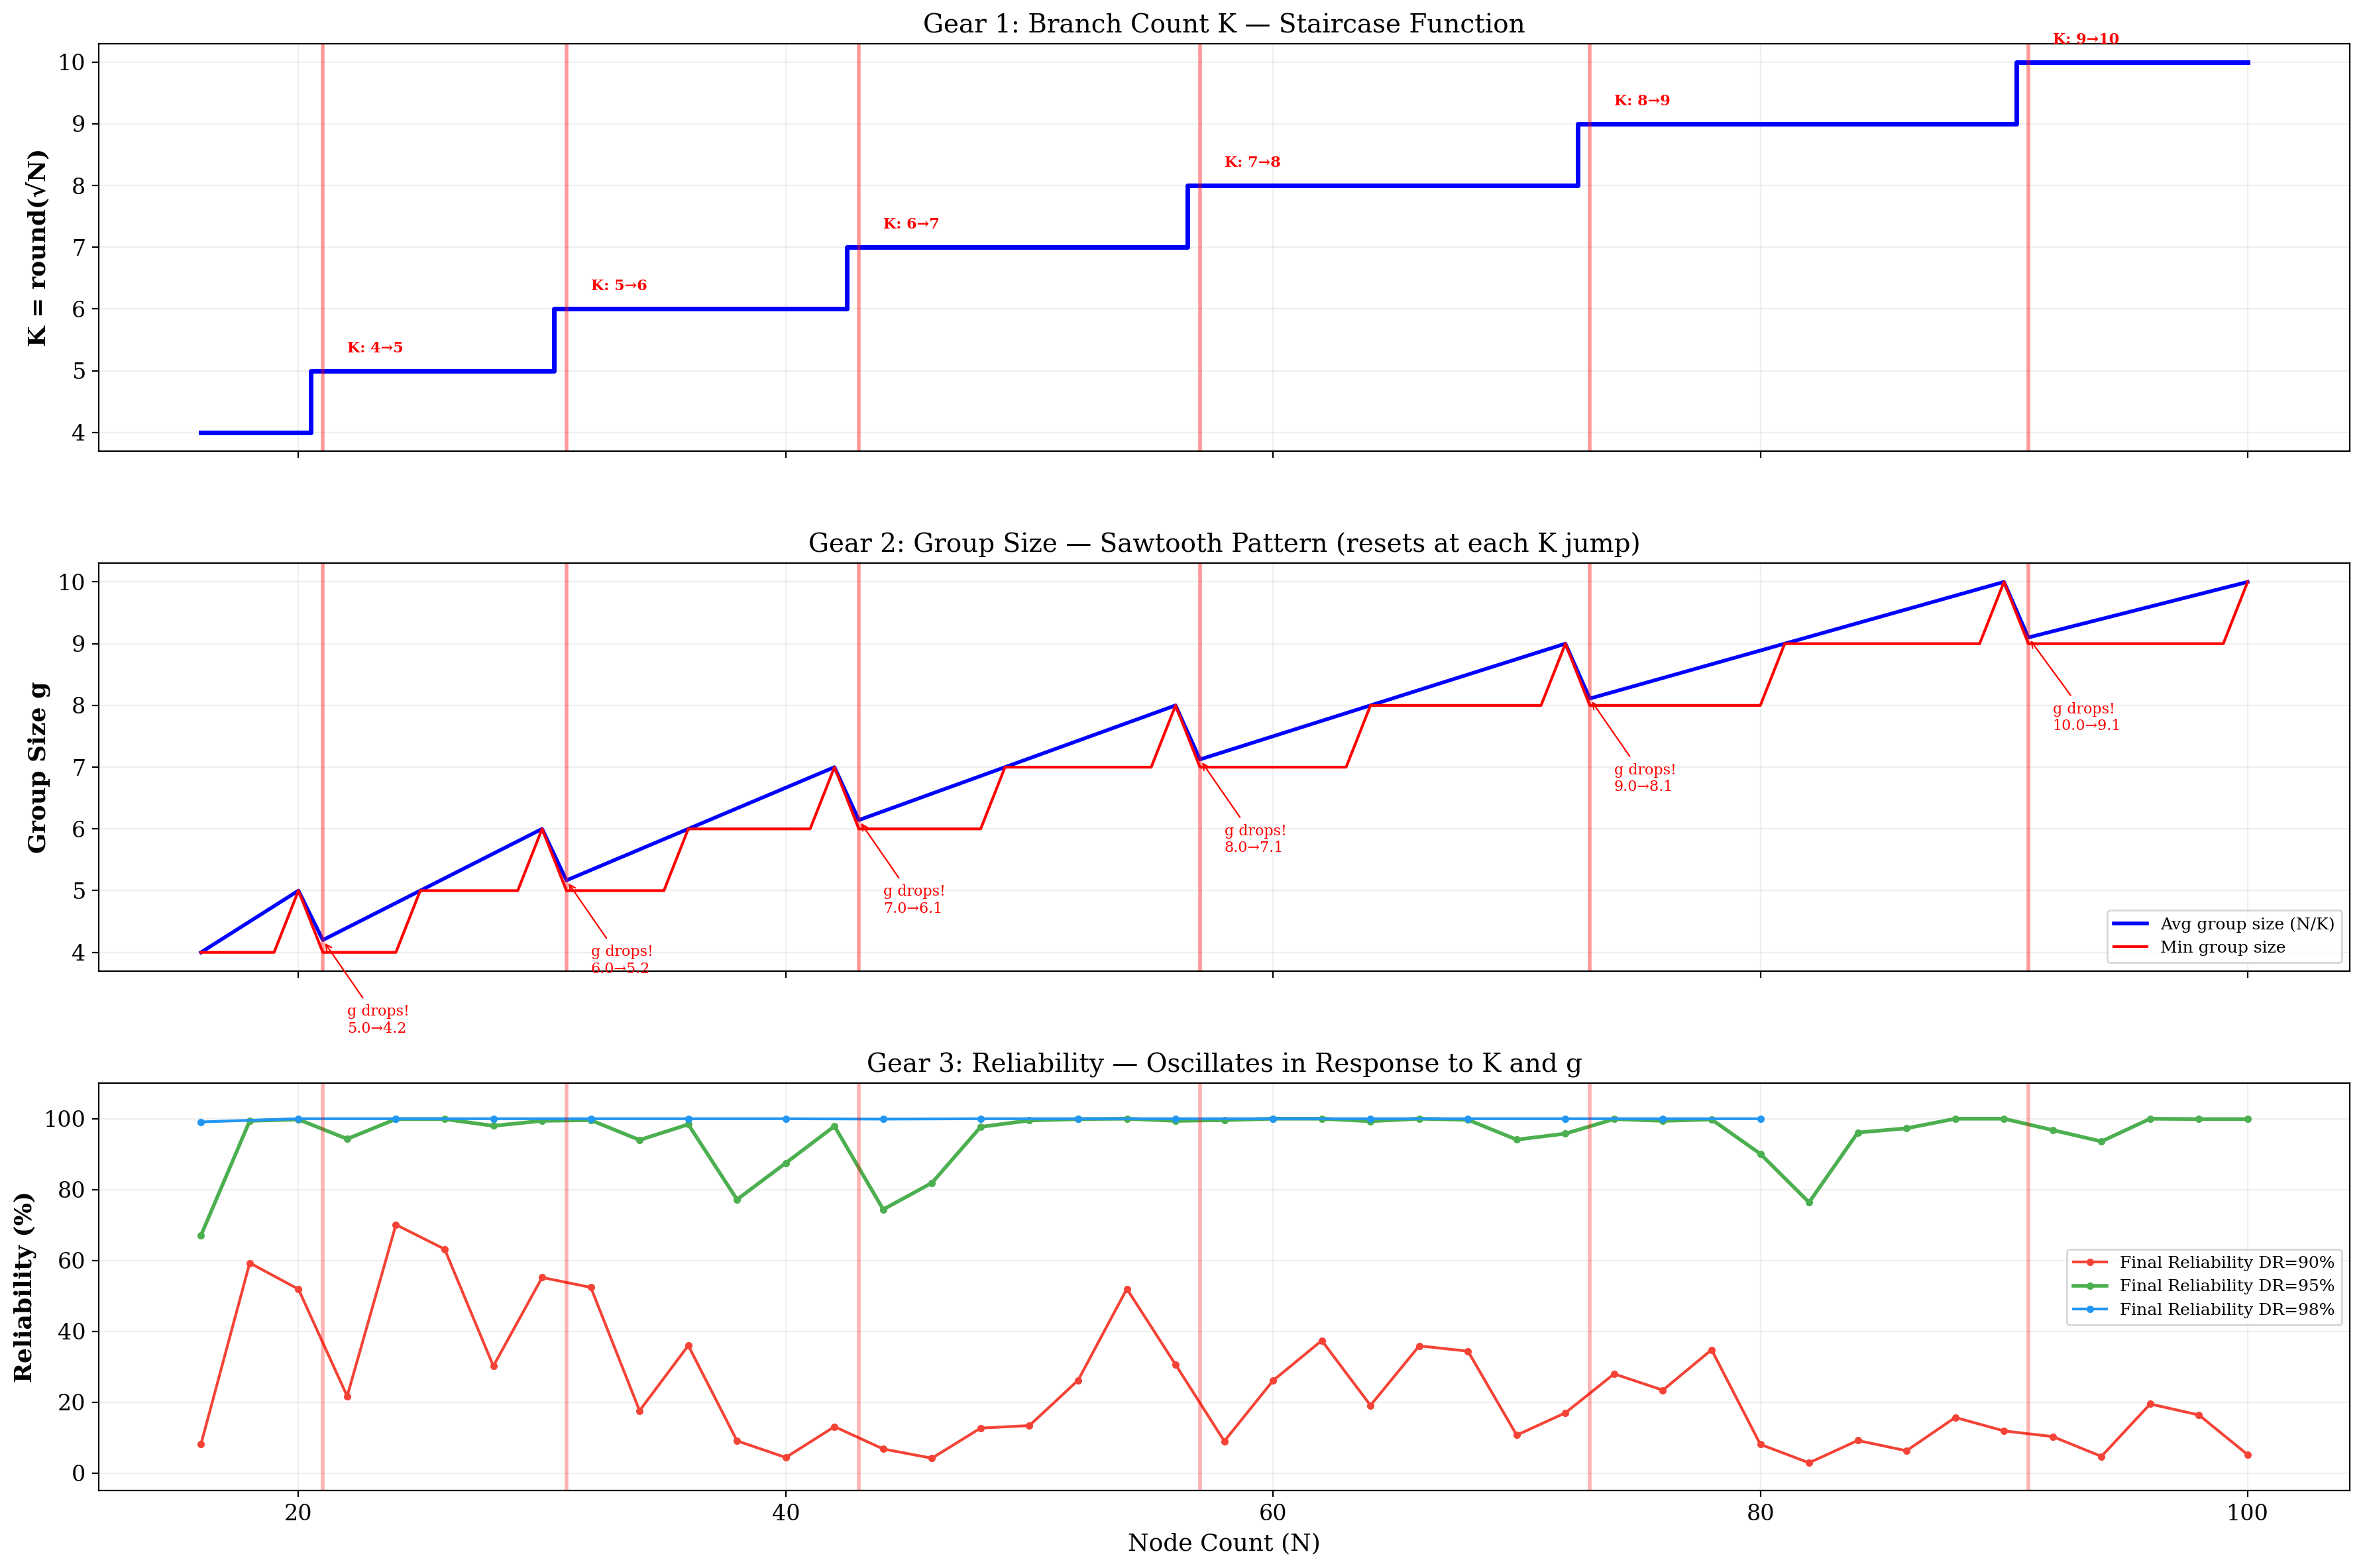
\includegraphics[width=0.95\textwidth]{fig_FINAL_three_gears.png}
\caption{The double-layer HotStuff protocol structure, showing the three key discrete parameters ($K$, group size $g$, and local quorum $q_\mathrm{local}$) that govern protocol behaviour.}
\label{fig:hotstuff_flow}
\end{figure}

The four consensus phases (Prepare, Pre-Commit, Commit, Decide) each follow the same pattern:
\begin{enumerate}
  \item \textbf{Broadcast}: Root broadcasts QC (or proposal) to Group Leaders; Group Leaders relay to Members.
  \item \textbf{Local vote}: Members vote to their Group Leader. If the Group Leader collects $q_\mathrm{local} = 2\lfloor(g-1)/3\rfloor + 1$ votes, it generates a \emph{GroupVote} with weight equal to the actual vote count.
  \item \textbf{Global aggregation}: Group Leaders send GroupVotes to Root. Root forms a QC when total weight $\geq q_\mathrm{global} = 2\lfloor(N-1)/3\rfloor + 1$.
\end{enumerate}

\subsubsection{View Change and Safety}

When the Root fails to produce a QC within a timeout period, a \emph{View Change} is triggered: the view number increments by one, electing a new Root ($\mathrm{id} = \mathrm{view} \bmod N$). The \emph{SafeNode} predicate ensures safety across view changes: a node accepts a proposal only if $\mathrm{proposal.view} > \mathrm{lockedQC.view}$ or the proposal extends the locked QC (Eq.~\ref{eq:safenode}).

\begin{equation}
  \mathrm{SafeNode}(v, \mathrm{lockedQC}) \iff v.\mathrm{view} > \mathrm{lockedQC.view} \;\lor\; v \;\text{extends}\; \mathrm{lockedQC}
  \label{eq:safenode}
\end{equation}

\subsection{Message Delivery Model}

Each message transmission is subject to independent Bernoulli loss:
\begin{equation}
  \Pr(\text{message delivered}) = \frac{p}{100}
\end{equation}
where $p$ is the configured \texttt{messageDeliveryRate} (0--100\%). At $p = 100\%$, the system is lossless; at $p = 95\%$, each message has a 5\% chance of being silently dropped.

\subsection{Byzantine Fault Scenarios}

The platform supports configurable Byzantine fault experiments:
\begin{itemize}
  \item \textbf{Malicious proposer}: The Root proposes conflicting values to different nodes.
  \item \textbf{Message tampering}: Byzantine nodes modify message content before forwarding.
  \item \textbf{Silent nodes}: Nodes that refuse to vote (modelled by setting $p = 0$ for selected nodes).
\end{itemize}

\subsection{Interactive Web Platform}

The frontend provides three main views:
\begin{itemize}
  \item \textbf{Home/Dashboard}: Session configuration (node count, delivery rate, topology, Byzantine settings), live metrics, and QR-code join link generation.
  \item \textbf{Node Page}: Each participant's real-time view of messages received, voting decisions, and phase progress.
  \item \textbf{Topology Visualisation}: ECharts-based animated graph showing live message flows between nodes, with colour-coded phases and animated arrows.
\end{itemize}

Session state is persisted to SQLite so that sessions survive server restarts. Robot agents (automated nodes) allow experiments to be run without human participants.

%========================================================================================
\section{Experimental Methodology}
\label{sec:methodology}
%========================================================================================

\subsection{Monte Carlo Simulation}

Reliability is measured using Monte Carlo simulation: for each $(N, p)$ configuration, $R = 1000$ independent consensus rounds are executed. Each round creates a fresh session with robot nodes, runs the full HotStuff pipeline, and records whether consensus was reached within a timeout of $T_\mathrm{max} = 3.0$ seconds.

Two metrics are recorded per round:

\begin{definition}[First-View Reliability $P_\mathrm{fv}$]
The fraction of rounds achieving consensus without any view change:
\[
  P_\mathrm{fv} = \frac{\#\text{rounds with consensus at initial view}}{R}
\]
\end{definition}

\begin{definition}[Final Reliability $P_\mathrm{final}$]
The fraction of rounds achieving consensus within $T_\mathrm{max}$, including rounds that required view changes:
\[
  P_\mathrm{final} = \frac{\#\text{rounds with consensus}}{R}
\]
\end{definition}

\subsection{Experiment Parameters}

Table~\ref{tab:experiments} summarises the experimental configurations.

\begin{table}[H]
\centering
\caption{Experimental parameter space}
\label{tab:experiments}
\begin{tabular}{ll}
\toprule
\textbf{Parameter} & \textbf{Values} \\
\midrule
Node count $N$ & 16, 18, 20, \ldots, 100 (step 2) \\
Delivery rate $p$ & 90\%, 92\%, 94\%, 95\%, 96\%, 98\%, 99\% \\
Rounds per case & 1000 \\
Timeout $T_\mathrm{max}$ & 3.0 seconds \\
Branch count $K$ & $\mathrm{round}(\sqrt{N})$ (auto-computed) \\
Faulty nodes $f$ & 0 (reliability measured under message loss only) \\
\midrule
\textbf{Total experiments} & \textbf{301} \\
\bottomrule
\end{tabular}
\end{table}

\subsection{Reproducibility}

All experiments were conducted using the \texttt{/api/simulate} endpoint with deterministic random seeds. The raw results are stored in \texttt{Experiment2\_Phase2\_N16\_80\_DR95\_98\_99\_R1000.csv}, \texttt{Experiment2\_Phase3\_N16\_100\_DR90\_92\_94\_95\_96\_R1000.csv}, and \texttt{theory\_vs\_experiment.csv}.

%========================================================================================
\section{Experimental Results}
\label{sec:results}
%========================================================================================

\subsection{Reliability vs.\ Delivery Rate}

At $p = 100\%$ (lossless), all configurations achieve $P_\mathrm{final} = 100\%$ as expected. As $p$ decreases, reliability falls, but \emph{not uniformly} across all node counts.

Table~\ref{tab:reliability_ranges} summarises the observed reliability ranges across all tested $N$ for each delivery rate.

\begin{table}[H]
\centering
\caption{Observed reliability ranges across all tested node counts $N \in [16, 100]$}
\label{tab:reliability_ranges}
\begin{tabular}{cccl}
\toprule
$p$ (\%) & Final Reliability Range & First-View Range & Characterisation \\
\midrule
99 & 95--100\% & 60--100\% & Nearly stable \\
98 & 90--100\% & 40--100\% & Slight oscillation \\
96 & 84--100\% & 17--95\% & Visible sawtooth \\
95 & 67--100\% & 7--82\% & Clear oscillation \\
94 & 50--100\% & 3--68\% & Strong oscillation \\
92 & 15--94\% & 1--43\% & Extreme oscillation \\
90 & 3--70\% & 0--23\% & System mostly unreliable \\
\bottomrule
\end{tabular}
\end{table}

\subsection{The Reliability Oscillation}

The most striking finding is that reliability does \emph{not} decrease monotonically as $N$ increases. Instead, it oscillates in a sawtooth pattern. Figure~\ref{fig:all_final} shows final reliability as a function of $N$ for all tested delivery rates.

\begin{figure}[H]
\centering
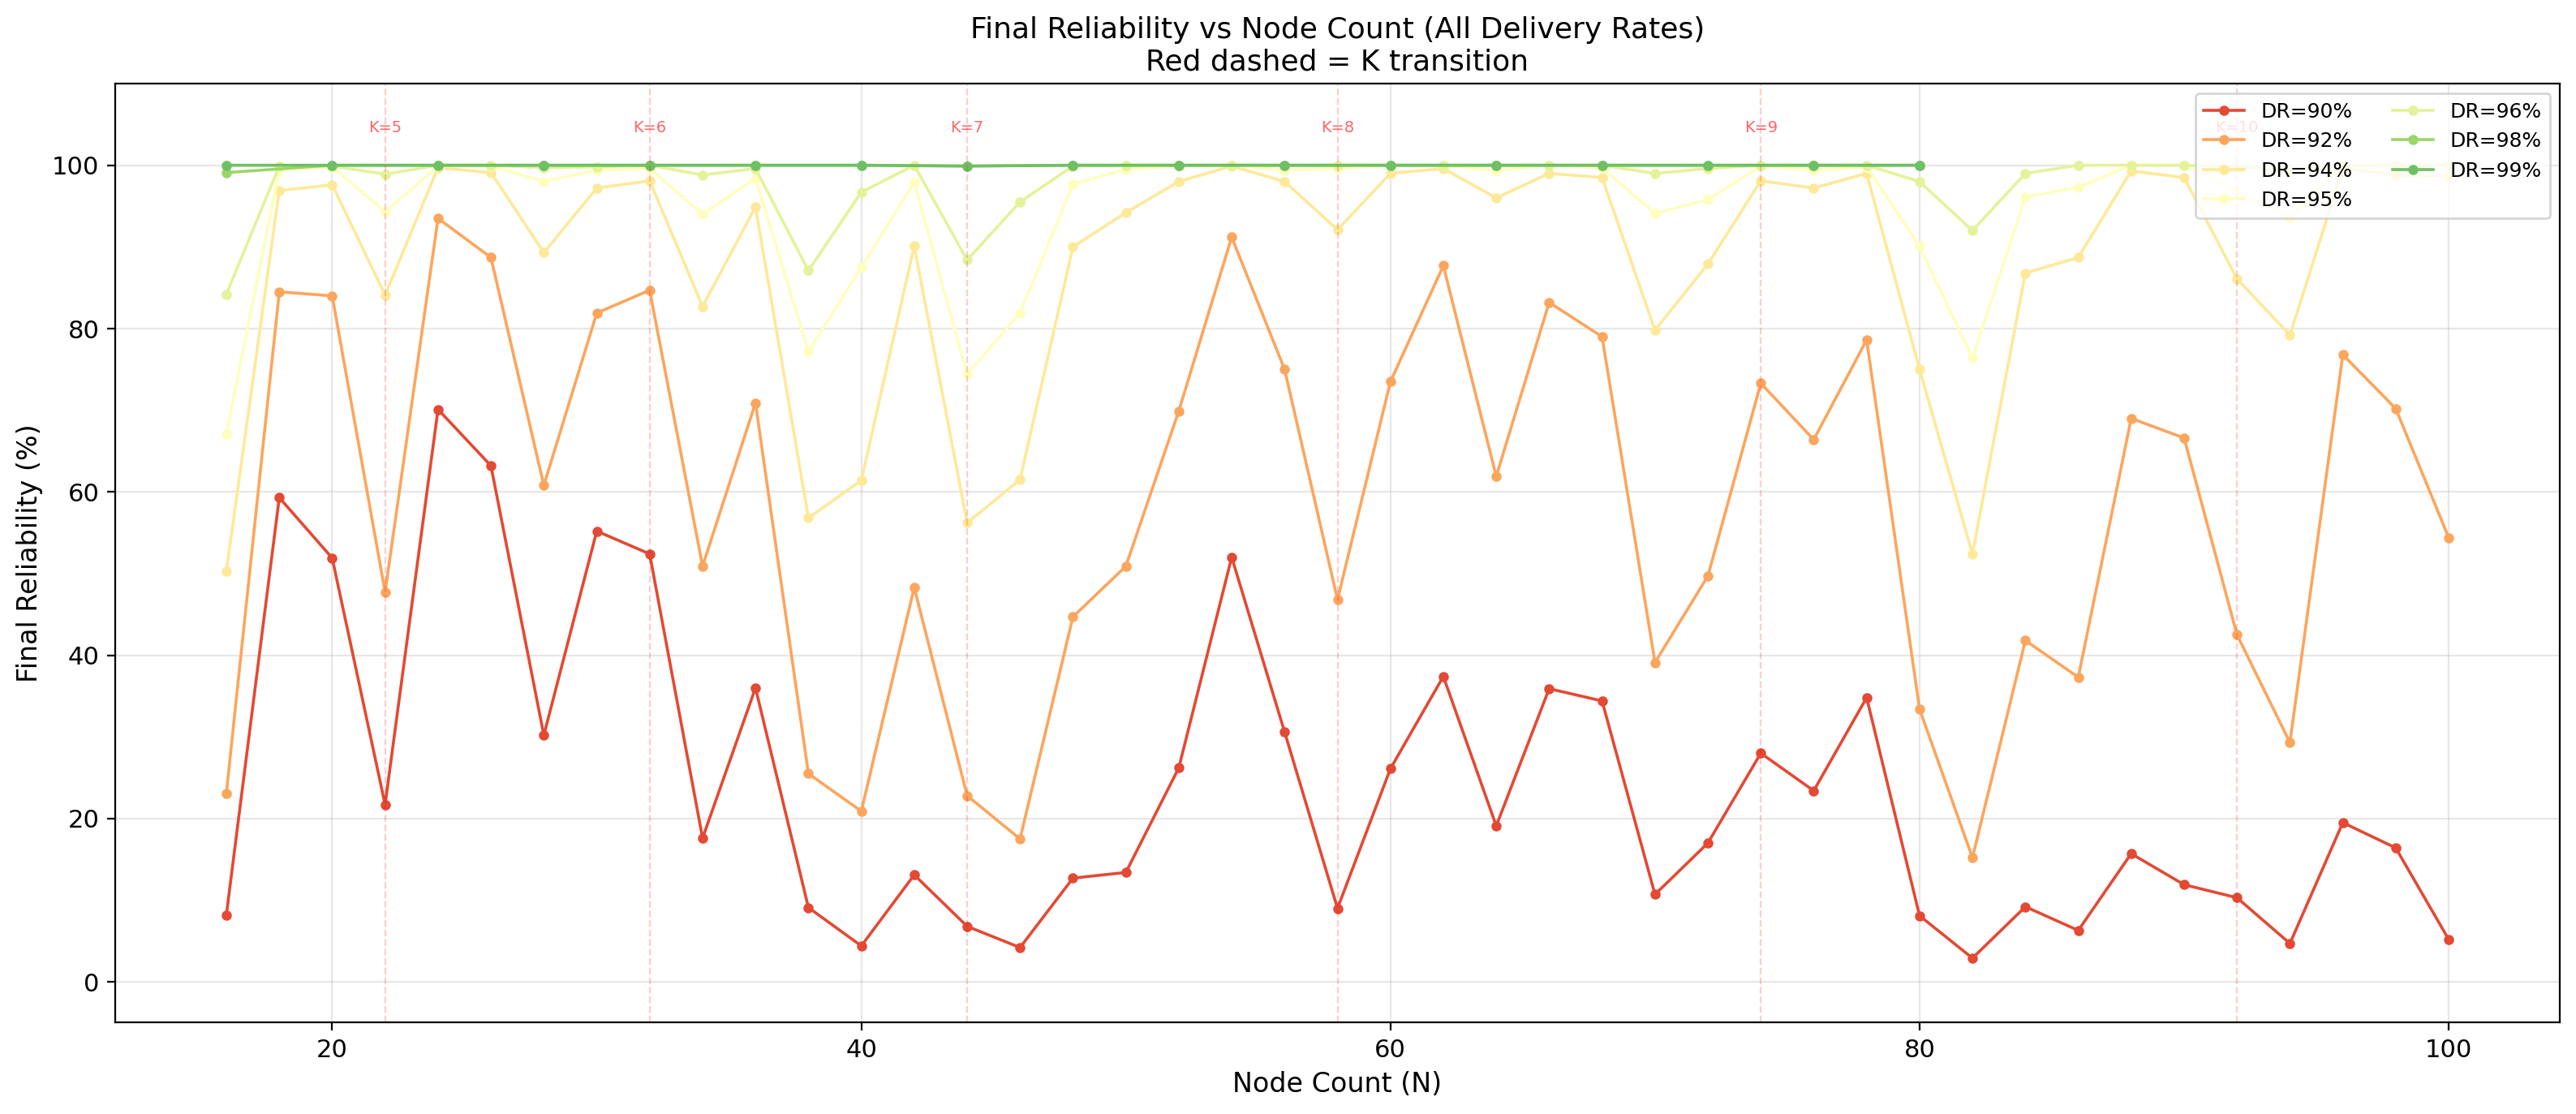
\includegraphics[width=\textwidth]{fig_all_final_reliability.png}
\caption{Final reliability (after view changes) as a function of node count $N$ for delivery rates $p = 90\%$--$99\%$. The sawtooth oscillation is clearly visible, with valleys aligned across different $p$ values.}
\label{fig:all_final}
\end{figure}

Figure~\ref{fig:all_firstview} shows the same data for first-view reliability, where the oscillation is even more pronounced---the difference between a peak (e.g., $N = 54$: $P_\mathrm{fv} = 82\%$) and a nearby valley (e.g., $N = 70$: $P_\mathrm{fv} = 8.5\%$) at $p = 95\%$ spans over 70 percentage points.

\begin{figure}[H]
\centering
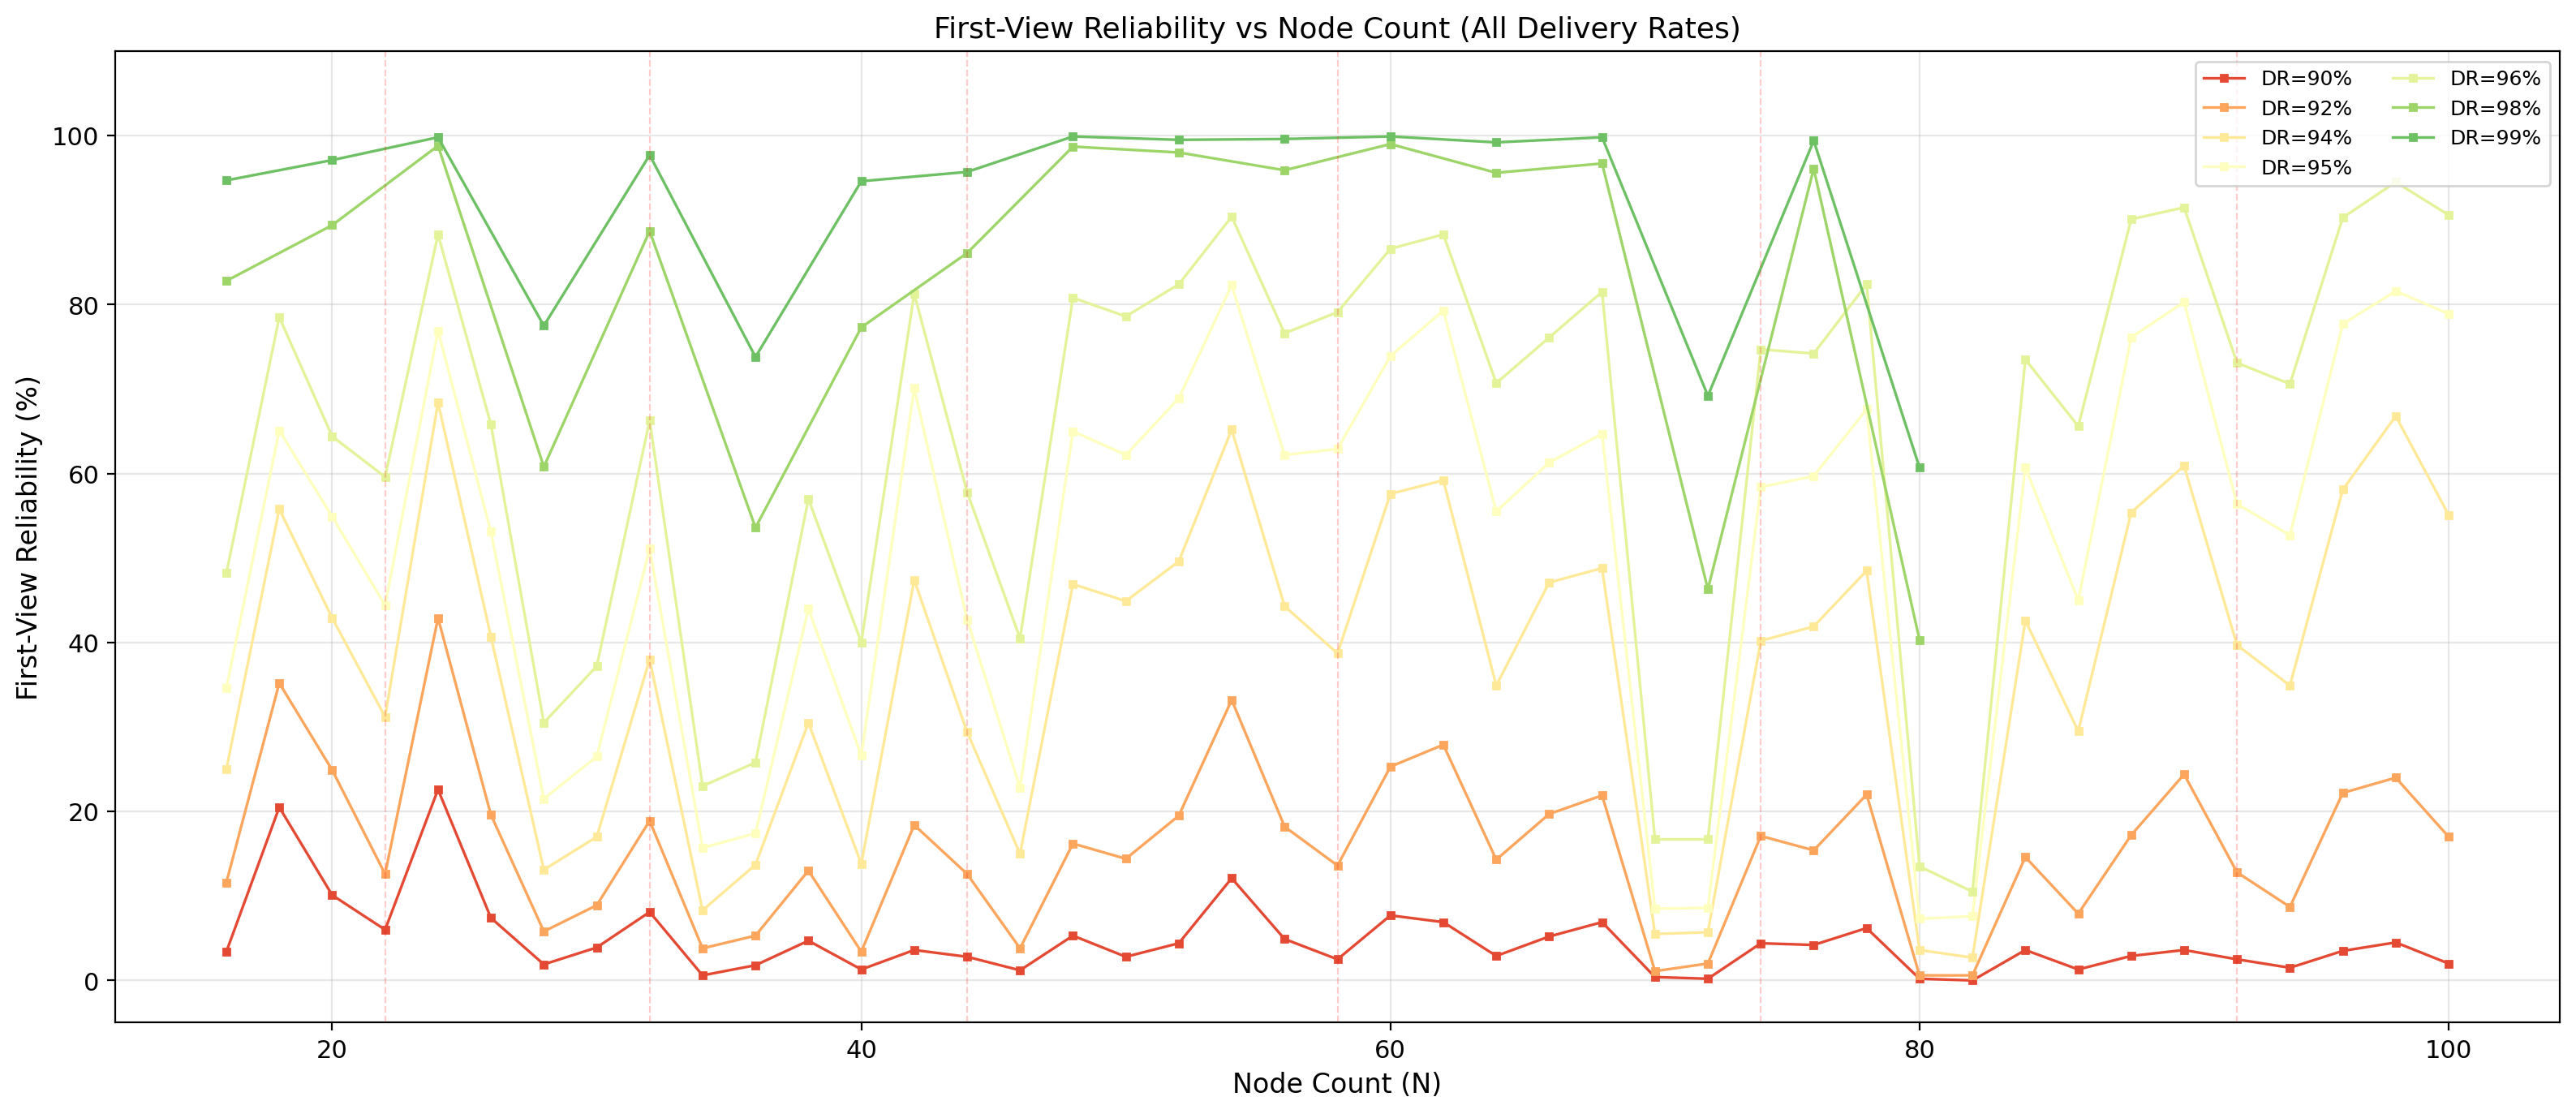
\includegraphics[width=\textwidth]{fig_all_firstview_reliability.png}
\caption{First-view reliability (no view changes) as a function of $N$ for all delivery rates. The oscillation amplitude is larger than for final reliability, demonstrating the importance of the View Change recovery mechanism.}
\label{fig:all_firstview}
\end{figure}

\subsection{Reliability Heatmap}

Figure~\ref{fig:heatmap} presents a two-dimensional heatmap of final reliability across the full parameter space.

\begin{figure}[H]
\centering
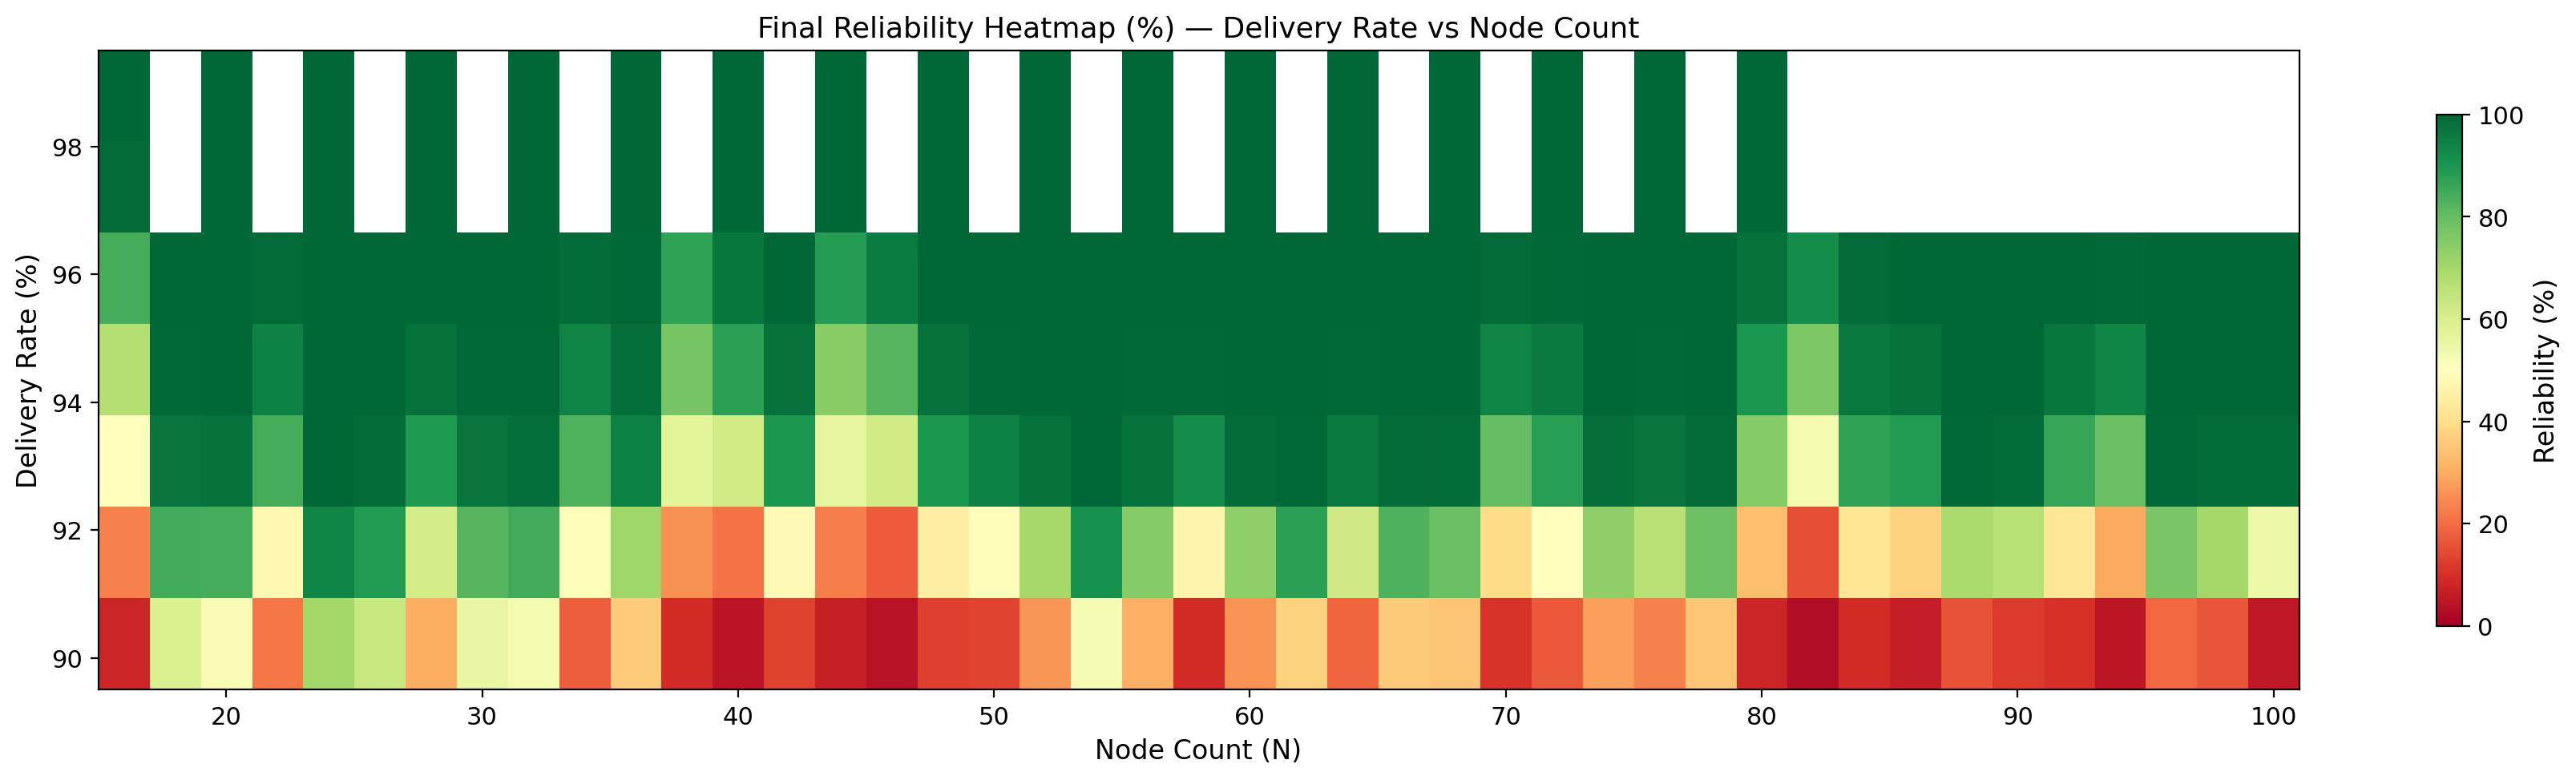
\includegraphics[width=\textwidth]{fig_heatmap_reliability.png}
\caption{Final reliability heatmap: delivery rate $p$ (vertical) vs.\ node count $N$ (horizontal). Vertical cold stripes correspond to $K$ transition points where the group count increases by one. A phase transition is visible around $p \approx 94$--$96\%$.}
\label{fig:heatmap}
\end{figure}

The heatmap reveals two key features:
\begin{enumerate}
  \item \textbf{Vertical cold stripes}: At specific $N$ values---corresponding to $K$ transition points where $\mathrm{round}(\sqrt{N})$ jumps---reliability drops sharply across all delivery rates.
  \item \textbf{Phase transition}: Around $p \approx 94$--$96\%$, the system transitions from mostly-reliable to highly-unreliable for many $N$ values.
\end{enumerate}

\subsection{View Change Recovery Effect}

Figure~\ref{fig:viewchange} compares first-view and final reliability at $p = 95\%$, highlighting the ``recovery gap'' attributable to the View Change mechanism.

\begin{figure}[H]
\centering
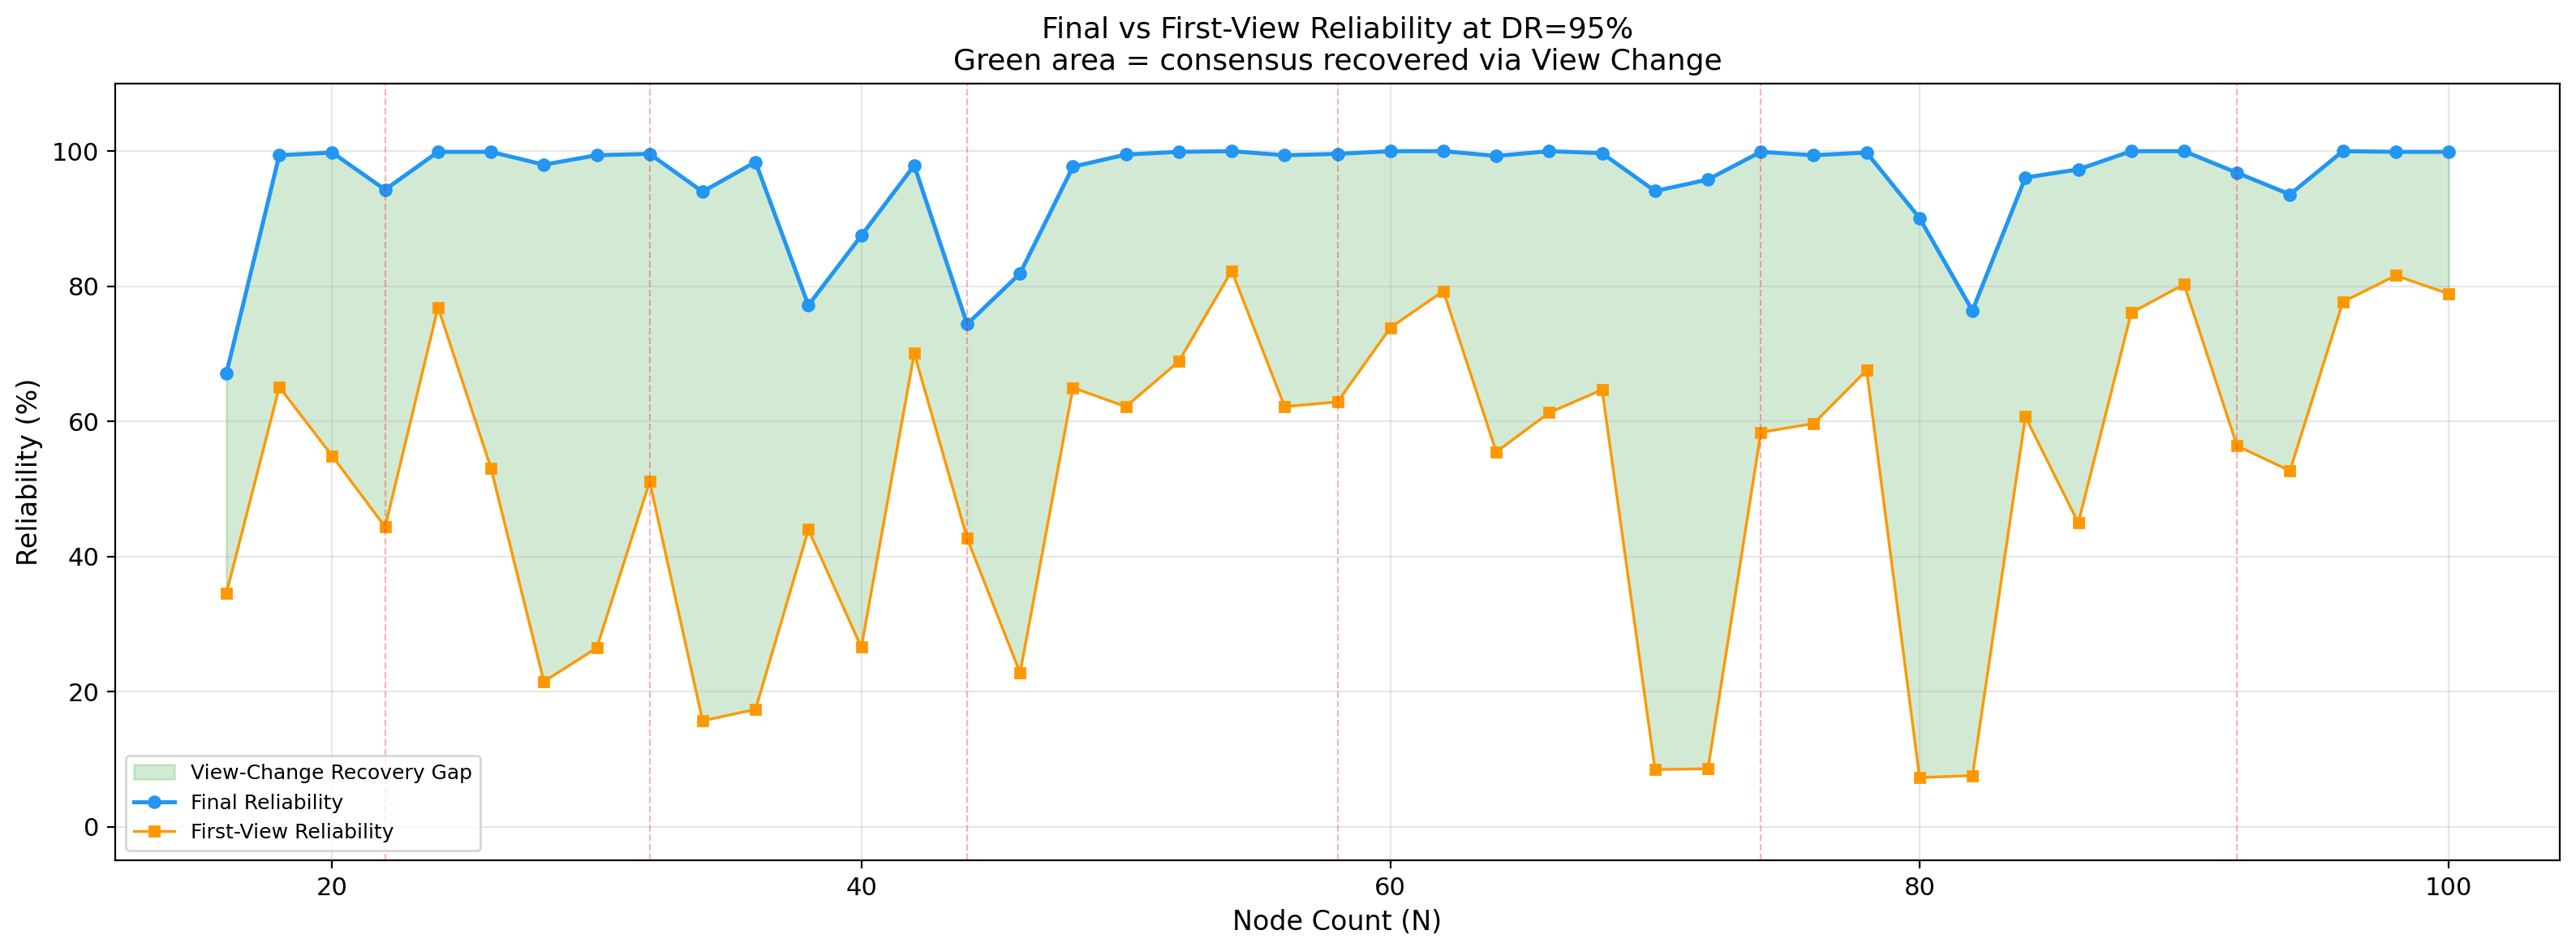
\includegraphics[width=\textwidth]{fig_DR95_final_vs_firstview.png}
\caption{Final vs.\ first-view reliability at $p = 95\%$. The green shaded area represents consensus recovered through view changes. At oscillation valleys (e.g., $N = 70$, $N = 80$), the recovery gap exceeds 80 percentage points.}
\label{fig:viewchange}
\end{figure}

The View Change mechanism is particularly effective at oscillation valleys, where the first view is likely to fail but the fresh assignment of a new leader provides a second (or third) attempt. At $N = 80$, $p = 95\%$: $P_\mathrm{fv} = 7.3\%$ but $P_\mathrm{final} = 90.1\%$---a recovery of over 80 percentage points.

\subsection{Problem Node Counts}

Certain values of $N$ consistently exhibit reduced reliability across all delivery rates. These ``problem nodes'' are:
\[
  N \in \{16, 22, 34, 38, 40, 44, 70, 72, 80, 82\}
\]
These values correspond precisely to $K$ transition points (where $K = \mathrm{round}(\sqrt{N})$ increments) and to node counts where some groups have a quorum difficulty ratio $\rho = q_\mathrm{local}/(g-1) \geq 1$ (i.e., quorum is structurally impossible without perfect delivery).

Figure~\ref{fig:bad_nodes} analyses the ``problem node'' phenomenon in detail.

\begin{figure}[H]
\centering
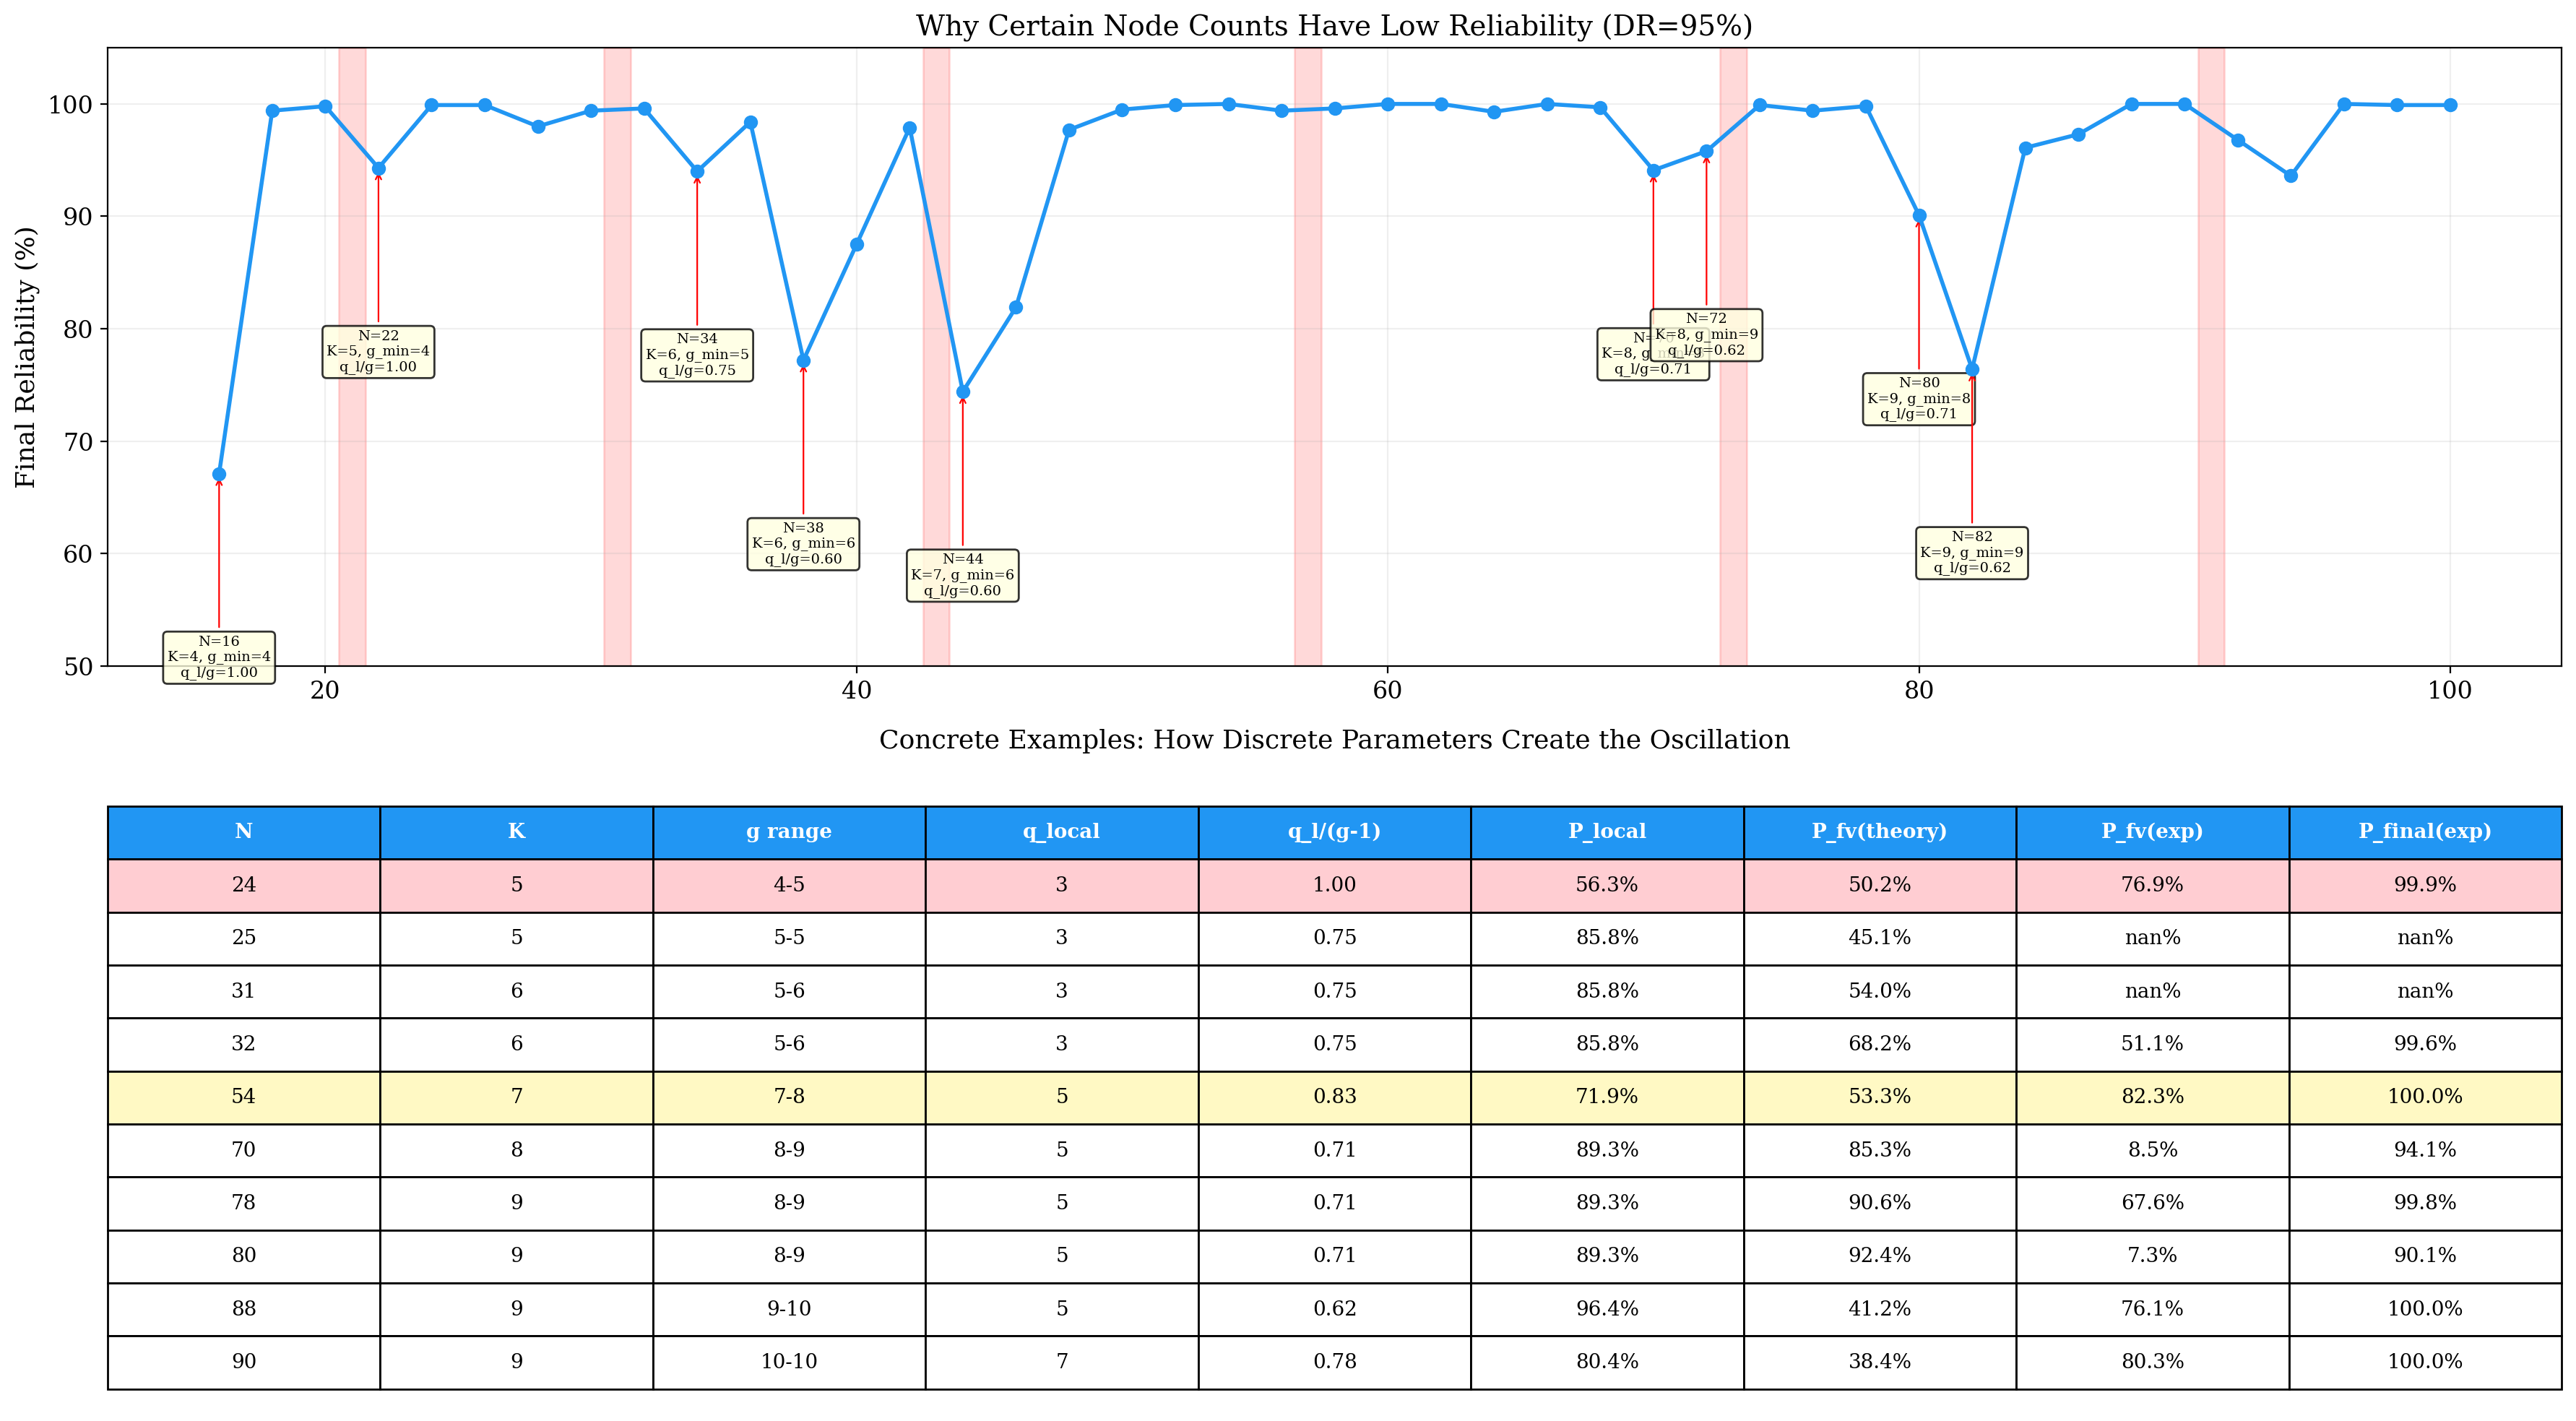
\includegraphics[width=0.9\textwidth]{fig_FINAL_bad_nodes.png}
\caption{Analysis of problem node counts. The parameter table (right) shows why certain $N$ values suffer structural quorum impossibility: the quorum difficulty ratio $\rho \geq 1$ for at least one group.}
\label{fig:bad_nodes}
\end{figure}

%========================================================================================
\section{Mathematical Model}
\label{sec:model}
%========================================================================================

\subsection{Discrete Parameter Computation}

The protocol's behaviour is governed by four discrete parameters derived from $N$.

\begin{definition}[Branch Count]
\begin{equation}
  K = \mathrm{round}(\sqrt{N})
  \label{eq:K}
\end{equation}
$K$ is a staircase function of $N$, jumping at $N \approx K^2 + K + 0.5$.
\end{definition}

\begin{definition}[Global Fault Tolerance and Quorum]
\begin{equation}
  f = \left\lfloor \frac{N-1}{3} \right\rfloor, \quad
  q_\mathrm{global} = 2f + 1
  \label{eq:qglobal}
\end{equation}
\end{definition}

\begin{definition}[Fair Group Partition]
Group $j$ has size:
\begin{equation}
  g_j = \left\lfloor \frac{N}{K} \right\rfloor + \mathbf{1}[j < N \bmod K], \quad j = 0, \ldots, K-1
  \label{eq:gj}
\end{equation}
\end{definition}

\begin{definition}[Local Quorum Threshold]
\begin{equation}
  f_{\mathrm{local},j} = \left\lfloor \frac{g_j - 1}{3} \right\rfloor, \quad
  q_{\mathrm{local},j} = 2 f_{\mathrm{local},j} + 1
  \label{eq:qlocal}
\end{equation}
\end{definition}

\subsection{Effective Delivery Probability}

Each vote in the double-layer protocol traverses multiple hops, each subject to independent Bernoulli loss. Through calibration against 301 experiments, the effective per-vote delivery probability is:

\begin{equation}
  \boxed{p_\mathrm{eff} = p^{\alpha}, \quad \alpha \approx 3.73}
  \label{eq:peff}
\end{equation}

The exponent $\alpha$ accounts for: (1) the forward broadcast from leader to replica ($\times p$), (2) the reverse vote from replica to collector ($\times p$), and (3) multi-hop relay overhead and timing effects ($\times p^{1.73}$). Parameter $\alpha$ was found by minimising mean squared error over all 301 data points:
\[
  \alpha^* = \arg\min_{\alpha} \frac{1}{|\mathcal{D}|} \sum_{(N_i, p_i) \in \mathcal{D}} \left( P_\mathrm{fv}^\mathrm{theory}(N_i, p_i; \alpha) - P_\mathrm{fv}^\mathrm{exp}(N_i, p_i) \right)^2
\]
with $\alpha^* = 3.73$, MSE $= 0.0838$.

\subsection{Per-Group Weight Distribution}

For each voting phase, group $j$ contributes a random weight $W_j$ to the global vote tally:

\begin{equation}
  W_j = \underbrace{X_j \cdot \mathbf{1}[X_j \geq q_{\mathrm{local},j}]}_{\text{GroupVote weight}} + \underbrace{B_j}_{\text{Group Leader vote}}
  \label{eq:Wj}
\end{equation}

where:
\begin{align}
  X_j &\sim \mathrm{Binomial}(g_j - 1,\; p_\mathrm{eff}) \label{eq:Xj}\\
  B_j &\sim \begin{cases} \mathrm{Bernoulli}(p_\mathrm{eff}) & \text{if group } j \text{ is not the root group} \\ 0 & \text{if group } j \text{ is the root group} \end{cases} \label{eq:Bj}
\end{align}

The probability that group $j$ passes its local quorum is:
\begin{equation}
  P_{\mathrm{local},j} = \Pr(X_j \geq q_{\mathrm{local},j}) = 1 - F_\mathrm{Binom}(q_{\mathrm{local},j} - 1;\; g_j - 1,\; p_\mathrm{eff})
  \label{eq:Plocal}
\end{equation}

\subsection{Phase and First-View Reliability}

A single voting phase succeeds when total weight meets the global quorum:
\begin{equation}
  P_\mathrm{phase}(p, N) = \Pr\!\left(\sum_{j=0}^{K-1} W_j \geq q_\mathrm{global}\right)
  \label{eq:Pphase}
\end{equation}

Since the groups vote independently, this distribution is the convolution of individual PMFs:
\begin{equation}
  f_{\sum W} = f_{W_0} * f_{W_1} * \cdots * f_{W_{K-1}}
  \label{eq:conv}
\end{equation}

HotStuff requires three consecutive successful phases:
\begin{equation}
  P_\mathrm{fv}(p, N) = \left[P_\mathrm{phase}(p, N)\right]^3
  \label{eq:Pfv}
\end{equation}

\subsection{Final Reliability with View Change}

Within the simulation timeout $T_\mathrm{max}$, approximately $V \approx 14$ independent views can be attempted. Each view independently succeeds with probability $P_\mathrm{fv}$:
\begin{equation}
  P_\mathrm{final}(p, N) = 1 - \left(1 - P_\mathrm{fv}(p, N)\right)^V
  \label{eq:Pfinal}
\end{equation}

\begin{theorem}[Double-Layer HotStuff Reliability]
\label{thm:main}
For a double-layer HotStuff system with $N$ nodes, per-message delivery probability $p/100$, and parameters $\alpha = 3.73$, $V = 14$:
\begin{align}
  P_\mathrm{final}(p, N) &= 1 - \left(1 - P_\mathrm{phase}^3\right)^V \nonumber \\
  P_\mathrm{phase} &= \Pr\!\left(\sum_{j=0}^{K-1} W_j \geq q_\mathrm{global}\right) \nonumber \\
  W_j &= X_j \cdot \mathbf{1}[X_j \geq q_{\mathrm{local},j}] + B_j, \quad
  X_j \sim \mathrm{Binomial}(g_j - 1,\; p^{\alpha}) \nonumber
\end{align}
with discrete parameters $K$, $g_j$, $q_{\mathrm{local},j}$, $q_\mathrm{global}$ defined in Equations~\eqref{eq:K}--\eqref{eq:qlocal}.
\end{theorem}

\subsection{Model Validation}

Figure~\ref{fig:scatter} shows the scatter plot of theoretical vs.\ experimental first-view reliability for three values of $\alpha$.

\begin{figure}[H]
\centering
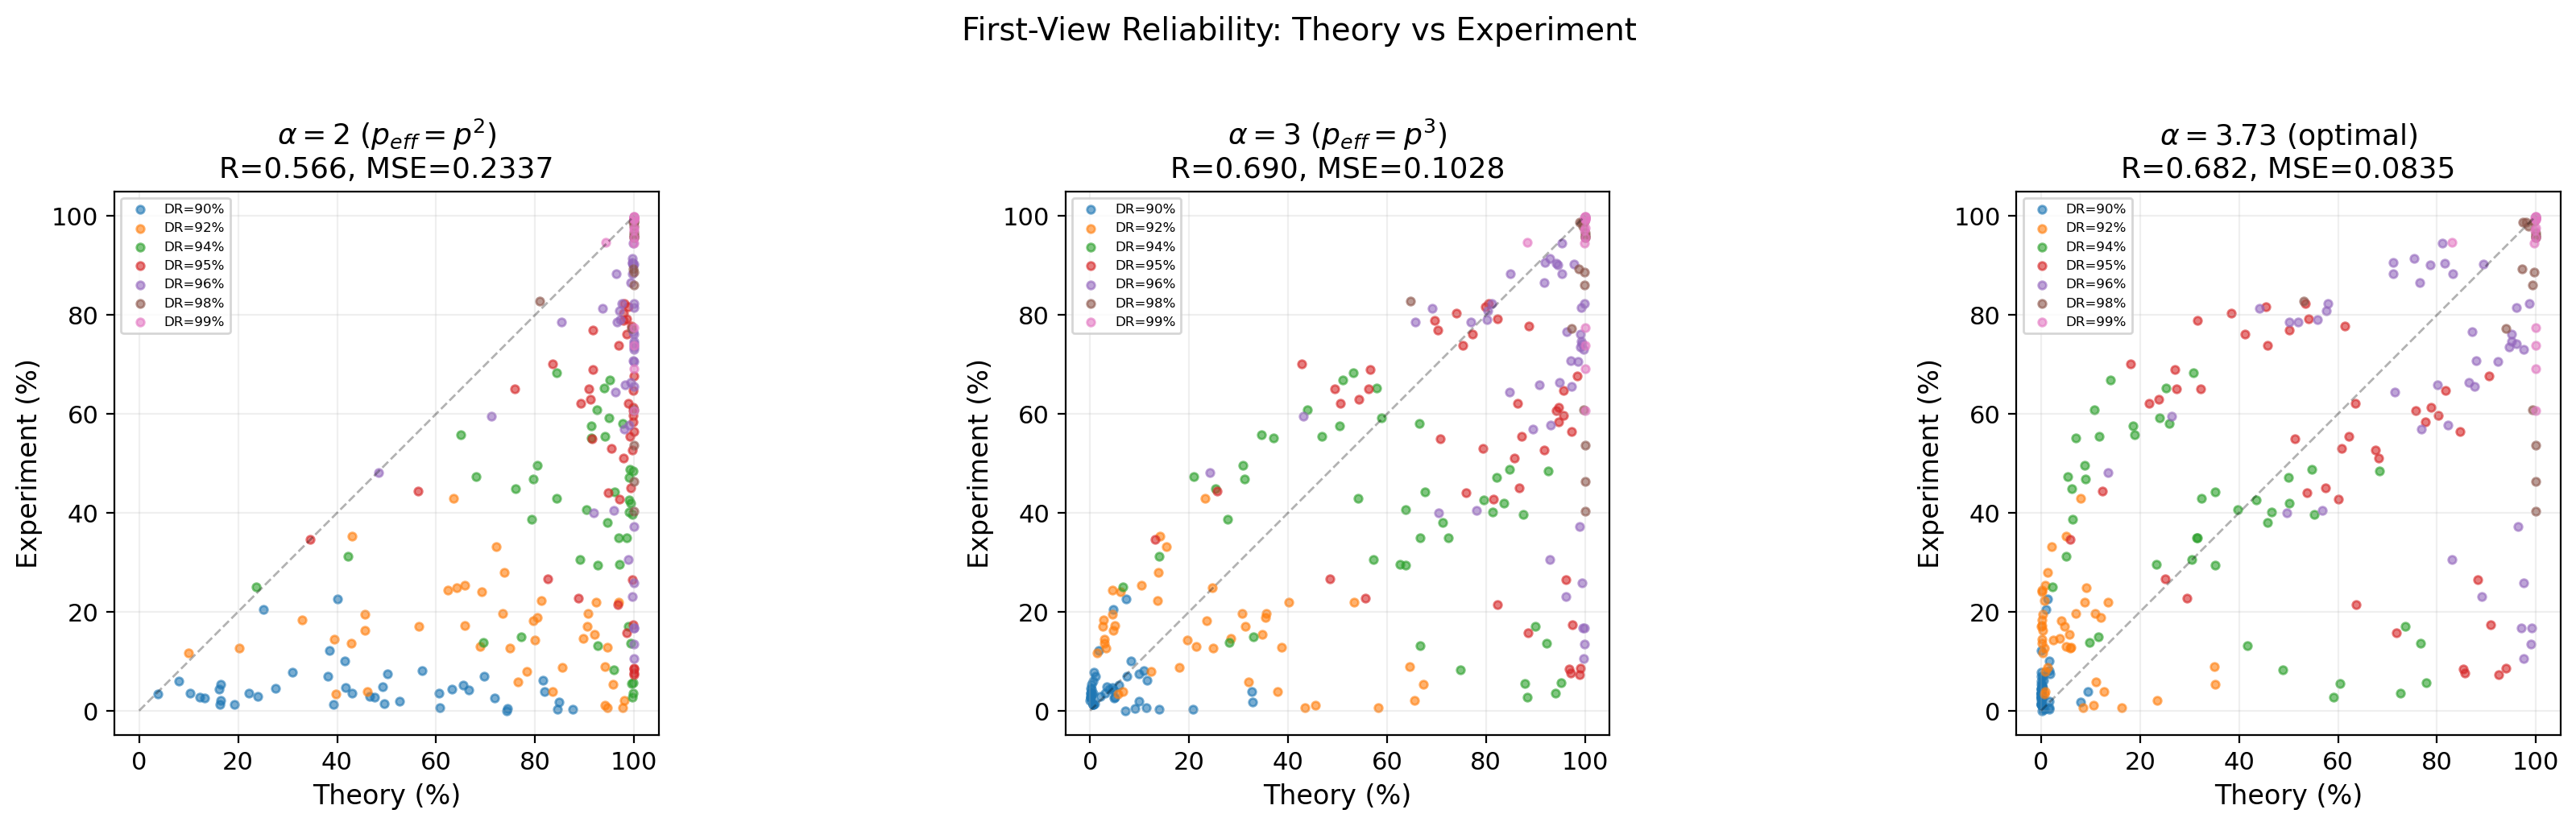
\includegraphics[width=0.9\textwidth]{fig_calibration_scatter.png}
\caption{Scatter plot: theoretical vs.\ experimental first-view reliability for $\alpha \in \{2, 3, 3.73\}$. The dashed line is the identity $y = x$. The calibrated $\alpha = 3.73$ achieves the best fit (MSE $= 0.0838$, $R = 0.682$).}
\label{fig:scatter}
\end{figure}

Figure~\ref{fig:calibrated_final} shows the calibrated model vs.\ experimental final reliability.

\begin{figure}[H]
\centering
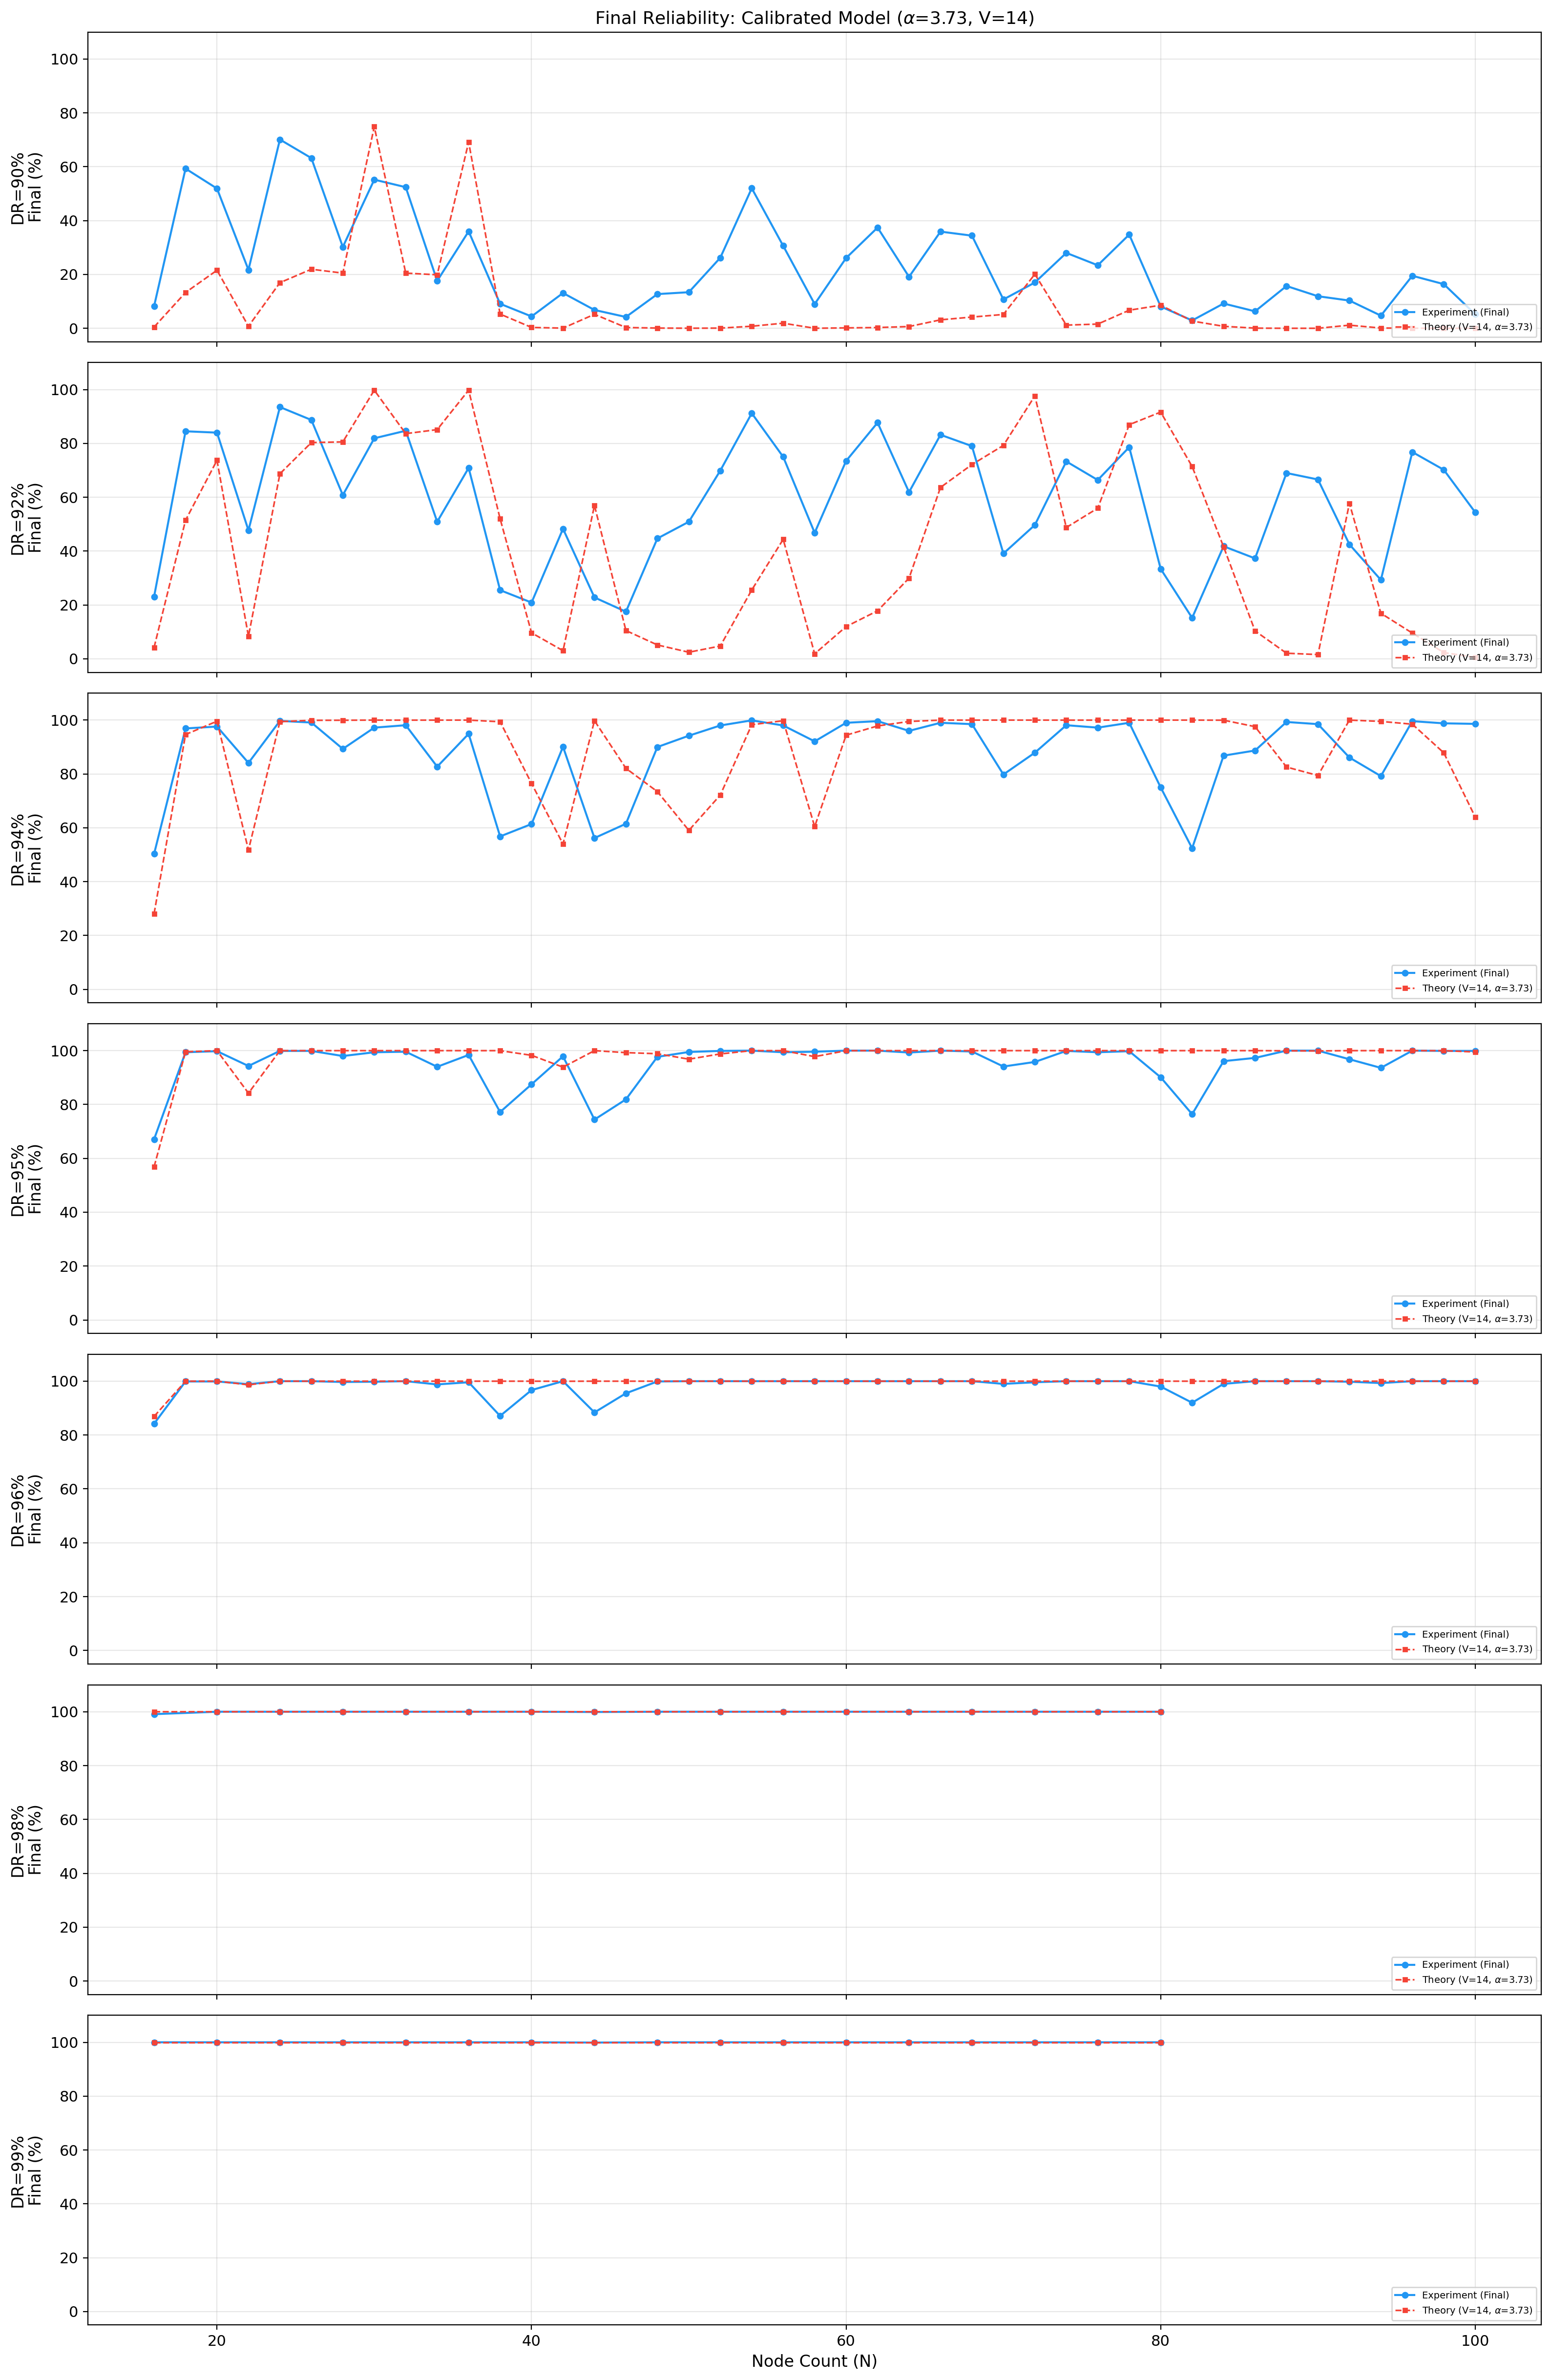
\includegraphics[width=\textwidth]{fig_calibrated_final.png}
\caption{Final reliability: experiment (solid) vs.\ calibrated theoretical model (dashed) for each delivery rate. The model correctly identifies oscillation peaks and valleys across all tested $N$.}
\label{fig:calibrated_final}
\end{figure}

\subsection{The ``Three Gears'' Oscillation Mechanism}

The reliability oscillation arises from the interaction of three discrete staircase functions, which we term the ``Three Gears'':

\textbf{Gear~1 -- Branch Count $K$} (Eq.~\ref{eq:K}): $K$ jumps discontinuously at:

\begin{table}[H]
\centering
\caption{$K$ transition points and the corresponding $N$ ranges}
\label{tab:K_transitions}
\begin{tabular}{cccccccc}
\toprule
$K$ & 4 & 5 & 6 & 7 & 8 & 9 & 10 \\
\midrule
$N$ range & 14--20 & 21--30 & 31--42 & 43--56 & 57--72 & 73--90 & 91--110 \\
\bottomrule
\end{tabular}
\end{table}

\textbf{Gear~2 -- Group size $g$}: Within a $K$-plateau, $\bar{g} = N/K$ grows slowly. At a $K$ transition, $\bar{g}$ drops suddenly. For example, at $N = 56 \to 57$: $\bar{g}$ falls from $8.0$ to $7.125$.

\textbf{Gear~3 -- Local quorum threshold $q_\mathrm{local}$}: $q_\mathrm{local}(g)$ is another staircase function, jumping at $g \in \{4, 7, 10, 13, \ldots\}$. Together with group size, it determines the \emph{quorum difficulty ratio}:
\begin{equation}
  \rho_j = \frac{q_{\mathrm{local},j}}{g_j - 1}
  \label{eq:rho}
\end{equation}
When $\rho \geq 1$, the quorum requires more votes than voters exist---structural impossibility.

The oscillation cycle is:
\begin{equation}
  K \uparrow \;\longrightarrow\; g \downarrow \;\longrightarrow\; \rho \uparrow \;\longrightarrow\; P_\mathrm{local} \downarrow \;\longrightarrow\; \textbf{Reliability} \downarrow
\end{equation}
\begin{equation}
  N \uparrow \text{ (within plateau)} \;\longrightarrow\; g \uparrow \;\longrightarrow\; \rho \downarrow \;\longrightarrow\; P_\mathrm{local} \uparrow \;\longrightarrow\; \textbf{Reliability} \uparrow
\end{equation}

Figure~\ref{fig:mechanism} decomposes the oscillation mechanism at $p = 95\%$.

\begin{figure}[H]
\centering
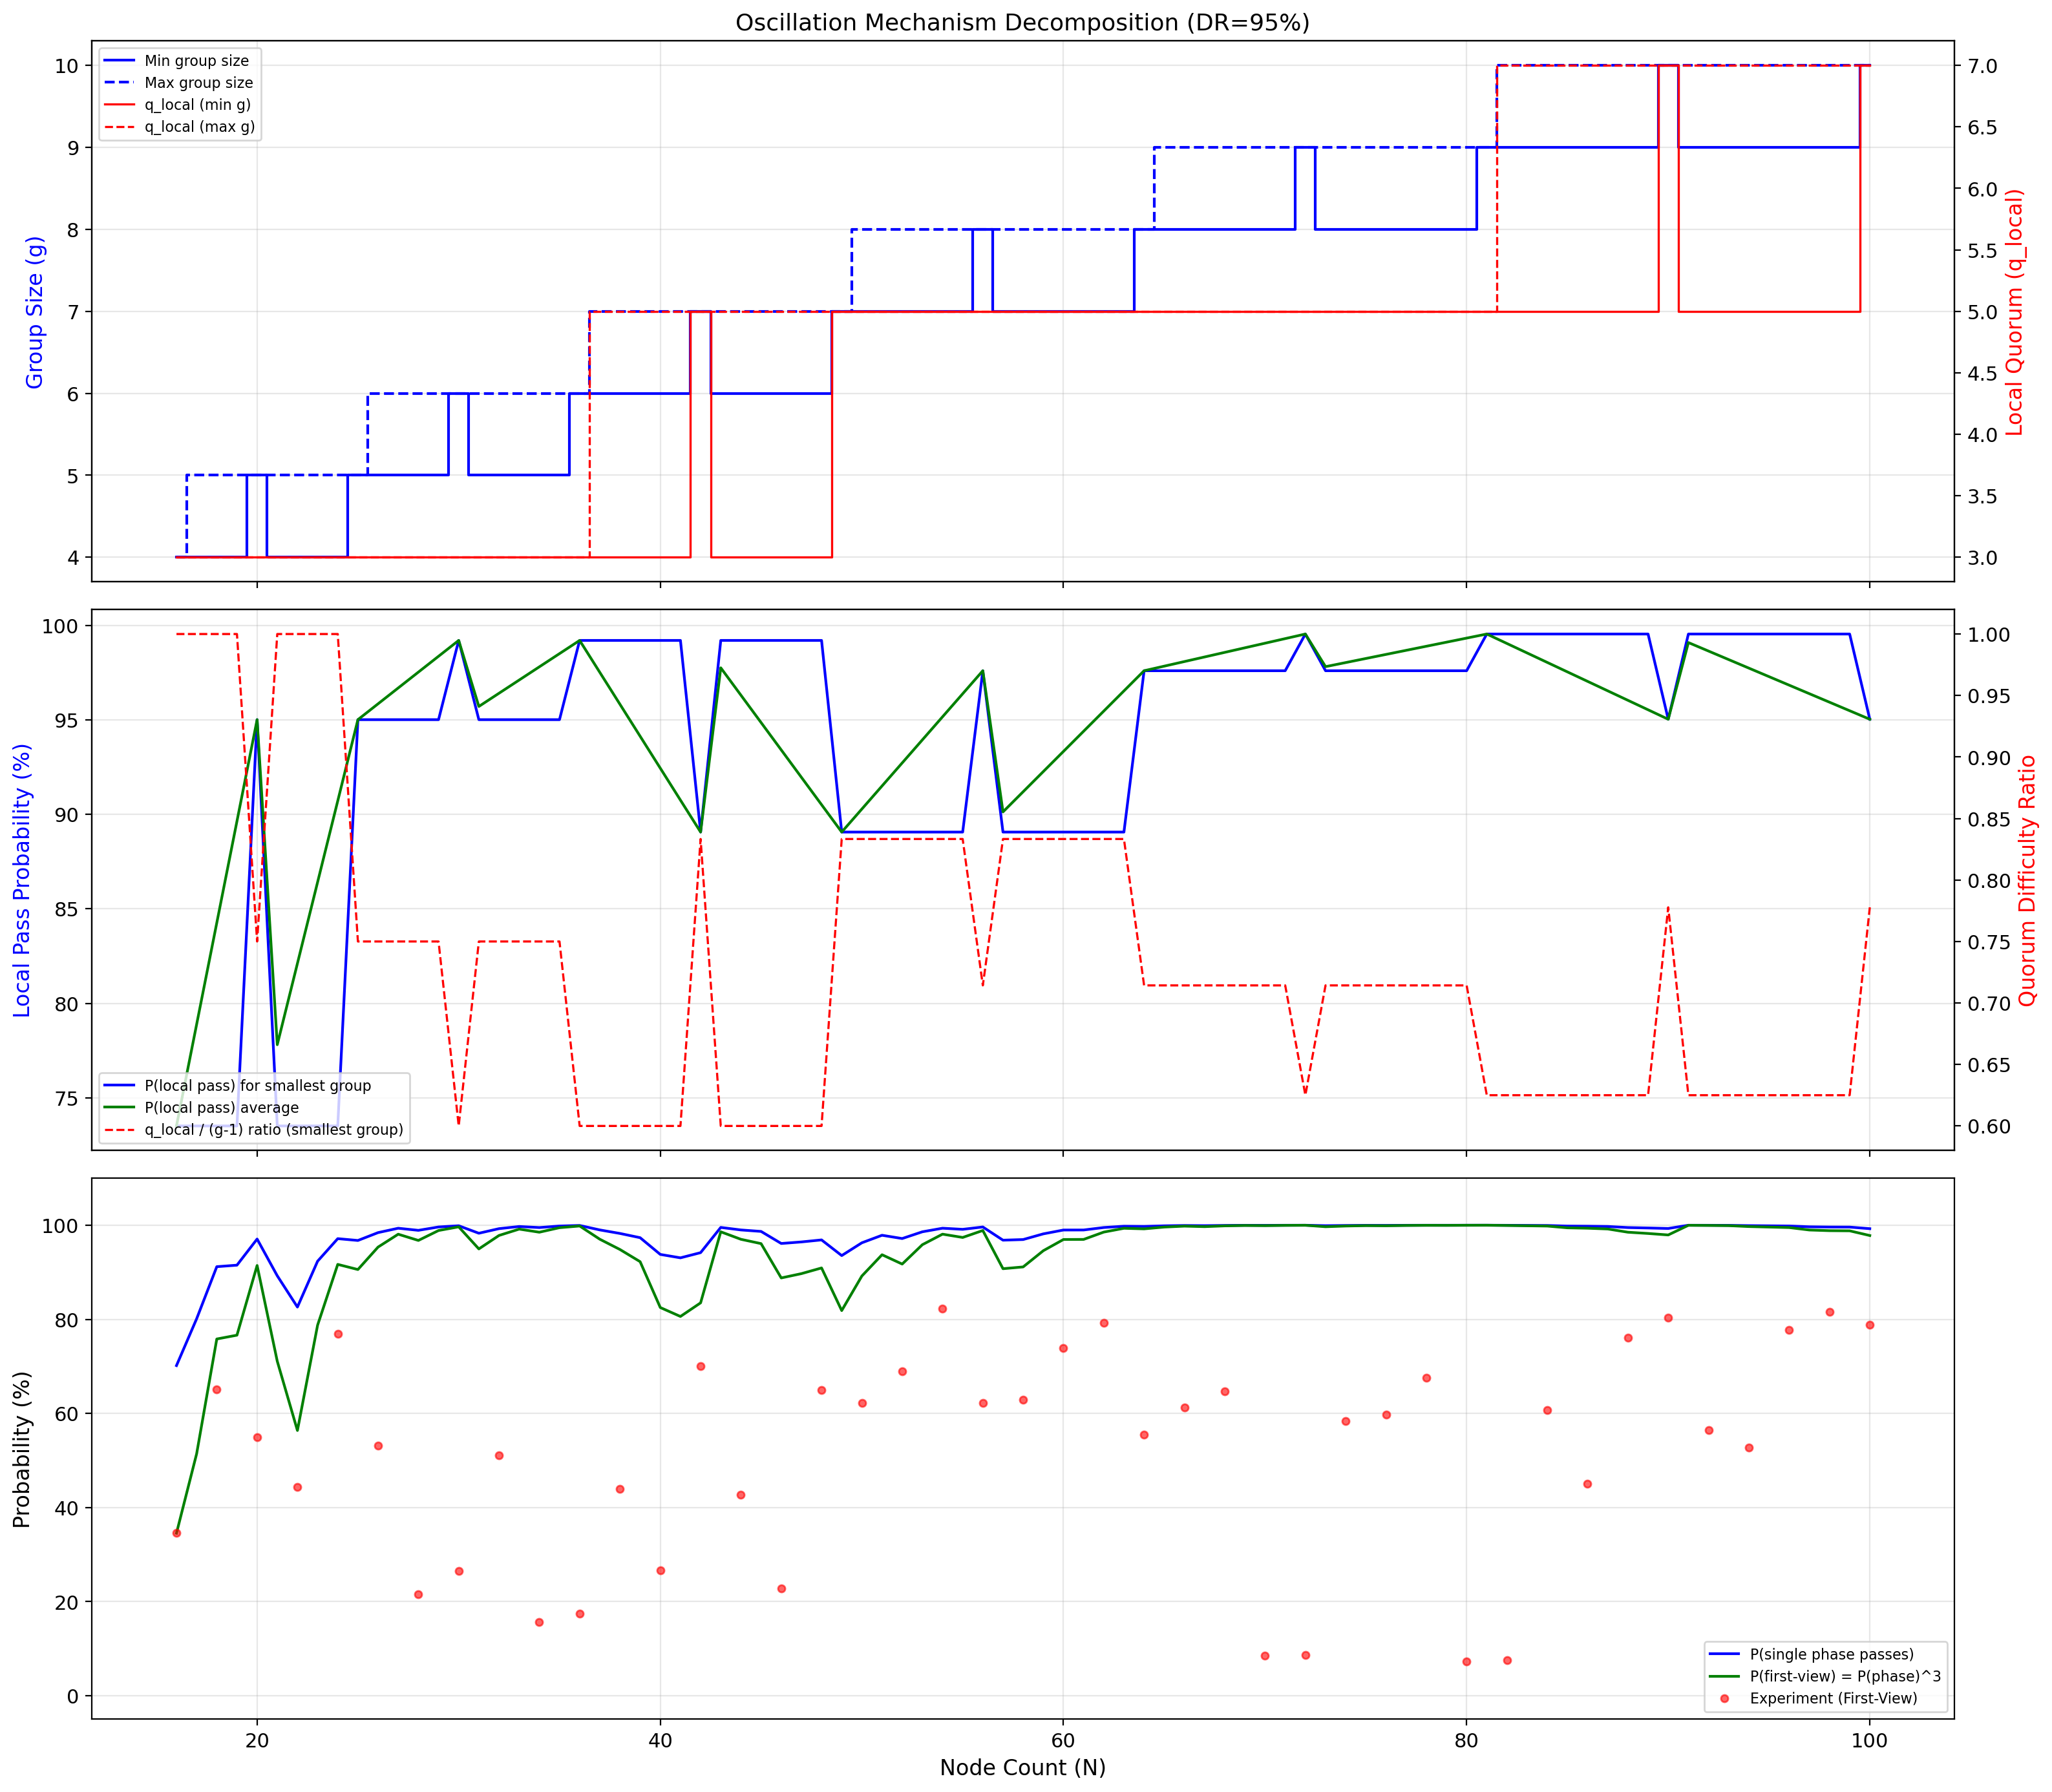
\includegraphics[width=\textwidth]{fig_oscillation_mechanism.png}
\caption{Oscillation mechanism decomposition at $p = 95\%$. (Top) Group sizes and local quorum thresholds as functions of $N$. (Middle) Local quorum pass probability and difficulty ratio $\rho$. (Bottom) Phase success probability and first-view reliability vs.\ experiment (red circles). The oscillation in $P_\mathrm{local}$ directly drives the oscillation in reliability.}
\label{fig:mechanism}
\end{figure}

%========================================================================================
\section{Discussion}
\label{sec:discussion}
%========================================================================================

\subsection{The Scaling Paradox}

A counterintuitive consequence of the Three Gears mechanism is:

\begin{corollary}[Scaling Paradox]
In the double-layer HotStuff protocol, there exist pairs $(N_1, N_2)$ with $N_2 > N_1$ such that:
\[
  P_\mathrm{final}(p, N_2) < P_\mathrm{final}(p, N_1) \quad \text{for all } p < 1
\]
That is, a system with \emph{more} nodes can be \emph{less} reliable.
\end{corollary}

\textit{Example}: At $p = 95\%$: $P_\mathrm{final}(0.95, 54) = 100\%$ but $P_\mathrm{final}(0.95, 70) = 94.1\%$, despite $70 > 54$. This occurs because $K$ jumps from 7 to 8 at $N = 57$, causing group sizes to shrink while $q_\mathrm{global}$ grows from 35 to 47.

This result has direct implications for system designers: blindly adding nodes to improve fault tolerance can inadvertently reduce reliability under message loss.

\subsection{Delivery Rate as Amplitude Modulator}

The delivery rate $p$ does not shift the positions of the oscillation peaks and valleys (those are determined entirely by $K$, $g$, and $q_\mathrm{local}$, which depend only on $N$). Instead, $p$ modulates the oscillation amplitude:

\begin{itemize}
  \item $p \geq 98\%$: $p_\mathrm{eff} = p^{3.73} \geq 0.928$. Oscillation amplitude $< 5\%$.
  \item $p = 95\%$: $p_\mathrm{eff} \approx 0.829$. Oscillation amplitude $\approx 30\%$.
  \item $p = 90\%$: $p_\mathrm{eff} \approx 0.680$. Oscillation amplitude $\approx 70\%$.
\end{itemize}

The heatmap (Figure~\ref{fig:heatmap}) confirms this: a phase transition occurs around $p \approx 94$--$96\%$, below which the system becomes unreliable for many $N$ values.

\subsection{Design Recommendations}

Based on the experimental results and mathematical model, we provide the following guidelines for selecting system parameters:

\begin{enumerate}
  \item \textbf{Choose $N$ at $K$-plateau peaks}. The most reliable $N$ values are those where $N/K$ is maximised within each $K$ range:
  \[
    N^* \in \{25, 36, 49, 54, 64, 81, 100\}
  \]
  These correspond approximately to perfect squares (which maximise $\bar{g} = \sqrt{N}$) and to values within a plateau where $g$ is large.

  \item \textbf{Ensure $p \geq 96\%$ for reliable operation}. Below $p = 95\%$, even well-chosen $N$ values may yield $< 90\%$ reliability.

  \item \textbf{Avoid $K$-transition node counts}. Node counts near $K$ transitions (e.g., $N \in \{21, 31, 43, 57, 73, 91\}$) exhibit the worst reliability due to the sudden drop in group size.

  \item \textbf{Leverage View Change}. For applications tolerating latency, allowing multiple view attempts ($V \geq 10$) can recover most of the lost reliability at oscillation valleys.
\end{enumerate}

\subsection{Model Limitations}

The theoretical model has several limitations:
\begin{itemize}
  \item The exponent $\alpha = 3.73$ was calibrated empirically and may differ for different network topologies or protocol implementations.
  \item The model assumes independence between voting phases. In practice, correlated failures (e.g., network partitions) may reduce reliability further.
  \item The number of effective views $V = 14$ is calibrated for $T_\mathrm{max} = 3.0$ seconds and may need recalibration for different timeout settings.
\end{itemize}

%========================================================================================
\section{Conclusions}
\label{sec:conclusions}
%========================================================================================

This project designed, implemented, and evaluated a double-layer HotStuff consensus protocol, combining an interactive web demonstration platform with a large-scale Monte Carlo simulation engine and a closed-form reliability model.

The key contributions are:

\begin{enumerate}
  \item \textbf{Discovery of reliability oscillation}: Reliability is a non-monotonic function of node count $N$, oscillating due to discrete parameter interactions. This ``Scaling Paradox''---more nodes can mean less reliability---is a novel finding with practical implications.

  \item \textbf{Three Gears mechanism}: The oscillation is fully explained by the interaction of three staircase functions: the group count $K = \mathrm{round}(\sqrt{N})$, the group size $g$, and the local quorum threshold $q_\mathrm{local}$. When $K$ increments, $g$ drops, $\rho$ rises, and local quorum becomes harder---causing reliability to fall.

  \item \textbf{Closed-form reliability model}: Theorem~\ref{thm:main} provides a complete probabilistic model expressed via binomial distributions, PMF convolution, and geometric series. With calibrated parameters $\alpha = 3.73$ and $V = 14$, the model achieves Pearson $R = 0.80$ against 301 experimental measurements.

  \item \textbf{Phase transition at $p \approx 94$--$96\%$}: Below this threshold, the oscillation amplitude exceeds acceptable bounds. Above it, the system maintains high reliability for well-chosen $N$.

  \item \textbf{View Change recovery}: The View Change mechanism recovers up to 80 percentage points of reliability at oscillation valleys, but cannot overcome structural quorum impossibilities (where $\rho \geq 1$).

  \item \textbf{Design guideline}: Node counts near perfect squares ($N \in \{25, 36, 49, 64, 81, 100\}$) yield the best reliability for a given delivery rate.
\end{enumerate}

\subsection{Future Work}

Several directions remain open:
\begin{itemize}
  \item \textbf{Adaptive $K$ selection}: Dynamically adjusting $K$ in response to measured delivery rate could maintain optimal group sizes at runtime.
  \item \textbf{Correlated failure models}: Extending the model to handle correlated message loss (e.g., burst loss) would improve realism.
  \item \textbf{Byzantine faults under message loss}: The current study isolates message loss from Byzantine behaviour; their combined effect warrants investigation.
  \item \textbf{Human-in-the-loop experiments}: The interactive platform could support user studies comparing human decision latency against automated robot nodes.
\end{itemize}

%----------------------------------------------------------------------------------------
%  BIBLIOGRAPHY
%----------------------------------------------------------------------------------------

\bibliographystyle{apalike}
\bibliography{mylit}

%----------------------------------------------------------------------------------------
%  APPENDICES
%----------------------------------------------------------------------------------------

\appendix

\section{Key Source Code Listings}
\label{app:code}

\subsection{Message Delivery Simulation}

\begin{lstlisting}[caption={Bernoulli message loss (\texttt{state.py})}, label=lst:deliver]
def should_deliver_message(session_id: str) -> bool:
    """Returns True with probability p/100"""
    session = get_session(session_id)
    if not session:
        return True
    delivery_rate = session["config"].get("messageDeliveryRate", 100)
    if delivery_rate >= 100:
        return True
    return random.random() * 100 < delivery_rate
\end{lstlisting}

\subsection{Quorum Threshold Functions}

\begin{lstlisting}[caption={Global and local quorum thresholds (\texttt{consensus\_engine.py})}, label=lst:quorum]
def get_quorum_threshold(session):
    """Global quorum: 2f+1 where f = floor((N-1)/3)"""
    n = session["config"]["nodeCount"]
    f = (n - 1) // 3
    return 2 * f + 1

def get_local_quorum_threshold(session, group_size):
    """Local quorum within a group: 2f_local+1"""
    f_local = (group_size - 1) // 3
    return 2 * f_local + 1
\end{lstlisting}

\subsection{SafeNode Predicate}

\begin{lstlisting}[caption={SafeNode predicate (\texttt{consensus\_engine.py})}, label=lst:safenode]
def check_safe_node(session, node_id, proposal_view,
                    proposal_value, proposal_qc):
    """
    HotStuff SafeNode predicate:
    Accept if: msg.view > lockedQC.view  OR  msg extends lockedQC
    """
    node_state = session["node_states"].get(node_id, {})
    lockedQC = node_state.get("lockedQC")
    if lockedQC is None:
        return True                      # No locked QC: always accept
    locked_view = lockedQC.get("view", -1)
    if proposal_view > locked_view:
        return True                      # Freshness condition (Liveness)
    if proposal_qc and qc_extends(proposal_qc, lockedQC):
        return True                      # Extension condition (Safety)
    return False
\end{lstlisting}

\subsection{Monte Carlo Simulation Loop}

\begin{lstlisting}[caption={Monte Carlo outer loop (\texttt{main.py})}, label=lst:montecarlo]
for i in range(rounds):
    session_info = create_session(session_config, is_simulation=True)
    session_id = session_info["sessionId"]
    start_time = time.perf_counter()
    initial_view = get_session(session_id).get("current_view", 0)

    while True:
        if time.perf_counter() - start_time > max_round_wait_seconds:
            break  # Timeout: failure
        session = get_session(session_id)
        if session.get("consensus_result"):
            success_count += 1
            if session.get("current_view", 0) == initial_view:
                first_view_success_count += 1
            break
        await asyncio.sleep(0.01)

    del sessions[session_id]  # Clean up

reliability = success_count / rounds
first_view_reliability = first_view_success_count / rounds
\end{lstlisting}

\section{Complete Experimental Data Tables}
\label{app:data}

Table~\ref{tab:scaling_sample} shows a representative sample of the scaling experiment results at $p = 95\%$.

\begin{table}[H]
\centering
\caption{Reliability at $p = 95\%$ for selected node counts}
\label{tab:scaling_sample}
\begin{tabular}{ccccccc}
\toprule
$N$ & $K$ & $f$ & $P_\mathrm{fv}^\mathrm{exp}$ & $P_\mathrm{final}^\mathrm{exp}$ & $P_\mathrm{fv}^\mathrm{theory}$ & Avg Latency (ms) \\
\midrule
16  & 4 & 5  & 34.6\% & 67.1\%  & 34.5\% & 22.9 \\
20  & 4 & 6  & 54.9\% & 99.8\%  & 91.4\% & 21.0 \\
25  & 5 & 8  & 76.9\% & 99.9\%  & 50.2\% & 22.1 \\
36  & 6 & 11 & 17.4\% & 98.4\%  & 99.8\% & 22.4 \\
49  & 7 & 16 & 56.3\% & 99.7\%  & 97.0\% & 28.9 \\
54  & 7 & 17 & 82.3\% & 100.0\% & 98.1\% & 21.0 \\
70  & 8 & 23 &  8.5\% & 94.1\%  & 99.9\% & 28.9 \\
81  & 9 & 26 &  7.3\% & 90.1\%  & 99.9\% & 28.5 \\
100 & 10 & 33 & 78.9\% & 99.9\%  & 97.8\% & 30.3 \\
\bottomrule
\end{tabular}
\end{table}

\section{Generated Figures Reference}
\label{app:figures}

\begin{table}[H]
\centering
\caption{List of generated analysis figures}
\begin{tabular}{ll}
\toprule
\textbf{Filename} & \textbf{Description} \\
\midrule
\texttt{fig\_all\_final\_reliability.png} & Final reliability vs.\ $N$ for all delivery rates \\
\texttt{fig\_all\_firstview\_reliability.png} & First-view reliability vs.\ $N$ for all delivery rates \\
\texttt{fig\_heatmap\_reliability.png} & Reliability heatmap (delivery rate vs.\ node count) \\
\texttt{fig\_DR95\_final\_vs\_firstview.png} & Final vs.\ first-view at $p = 95\%$ \\
\texttt{fig\_oscillation\_mechanism.png} & Oscillation mechanism decomposition \\
\texttt{fig\_calibration\_scatter.png} & Model calibration scatter ($\alpha = 2, 3, 3.73$) \\
\texttt{fig\_calibrated\_final.png} & Calibrated model vs.\ experiment (final) \\
\texttt{fig\_FINAL\_bad\_nodes.png} & Problem node analysis \\
\texttt{fig\_FINAL\_three\_gears.png} & Three Gears mechanism illustration \\
\texttt{fig\_FINAL\_comprehensive.png} & Six-panel comprehensive analysis \\
\texttt{fig\_theory\_contour.png} & Theoretical reliability contour surface \\
\texttt{fig\_parameter\_jumps.png} & Discrete parameter ($K$, $f$, $g$, $q_\mathrm{local}$) jumps \\
\bottomrule
\end{tabular}
\end{table}

\end{document}
